
\newpage
\section{Generalized Arrowhead Matrix Implementation}

This section describes the generalized implementation of the arrowhead matrix visualization and analysis. The implementation provides a unified interface for generating, analyzing, and visualizing arrowhead matrices of any size.

\subsection{Overview}

The generalized implementation combines the functionality of multiple scripts into a single, easy-to-use tool called \texttt{arrowhead.py}. This script serves as the main entry point for the arrowhead matrix implementation and provides a comprehensive set of features for matrix generation, eigenvalue/eigenvector calculation, and visualization.

\subsection{Key Features}

The generalized implementation provides the following key features:

\begin{itemize}
    \item \textbf{Unified Interface}: Combines the functionality of multiple scripts into a single, easy-to-use tool.
    \item \textbf{Flexible Parameters}: Allows customization of all important parameters, including origin vector, distance parameter, theta range, coupling constant, matrix size, and output directory.
    \item \textbf{Command-line Arguments}: Provides a comprehensive set of command-line options for easy use.
    \item \textbf{Multiple Operation Modes}: Supports full analysis, load-only mode, and plot-only mode.
    \item \textbf{Comprehensive Visualization}: Generates 2D eigenvalue plots, 3D eigenvector visualizations, and R vectors visualization.
\end{itemize}

\subsection{Usage}

The arrowhead matrix functionality can be accessed in two ways: directly through the \texttt{arrowhead.py} script or through the unified \texttt{main.py} interface.

\subsubsection{Using arrowhead.py}

The \texttt{arrowhead.py} script can be used directly as follows:

\begin{verbatim}
# Run with default parameters
python arrowhead.py

# Customize parameters
python arrowhead.py --size 6 --coupling 0.2 --theta-steps 36

# Only create plots from existing results
python arrowhead.py --plot-only

# Specify a custom output directory
python arrowhead.py --output-dir ./custom_results

# Specify perfect circle generation method (default is True)
python arrowhead.py --perfect
\end{verbatim}

\subsubsection{Using main.py}

Alternatively, you can use the unified \texttt{main.py} interface which provides access to both vector generation and arrowhead matrix functionality:

\begin{verbatim}
# Run with default parameters
python main.py arrowhead

# Customize parameters
python main.py arrowhead --size 6 --coupling 0.2 --theta-steps 36

# Only create plots from existing results
python main.py arrowhead --plot-only

# Specify a custom output directory
python main.py arrowhead --output-dir ./custom_results

# Specify perfect circle generation method (default is True)
python main.py arrowhead --perfect

# Show detailed help information
python main.py help
\end{verbatim}

The \texttt{main.py} interface provides a unified command-line interface for all functionality in the generalized arrowhead framework, including both vector generation and arrowhead matrix analysis.

\subsection{Command-line Arguments}

The script provides the following command-line arguments:

\begin{verbatim}
usage: arrowhead.py [-h] [--r0 R0 R0 R0] [--d D] [--theta-start THETA_START]
                    [--theta-end THETA_END] [--theta-steps THETA_STEPS]
                    [--coupling COUPLING] [--omega OMEGA] [--size SIZE]
                    [--output-dir OUTPUT_DIR] [--load-only] [--plot-only] [--perfect]

Arrowhead Matrix Generator and Analyzer

options:
  -h, --help            show this help message and exit
  --r0 R0 R0 R0         Origin vector (x, y, z)
  --d D                 Distance parameter
  --theta-start THETA_START
                        Starting theta value in radians
  --theta-end THETA_END
                        Ending theta value in radians
  --theta-steps THETA_STEPS
                        Number of theta values to generate matrices for
  --coupling COUPLING   Coupling constant for off-diagonal elements
  --omega OMEGA         Angular frequency for the energy term h*$\omega$
  --size SIZE           Size of the matrix to generate
  --output-dir OUTPUT_DIR
                        Directory to save results
  --load-only           Only load existing results and create plots
  --plot-only           Only create plots from existing results
\end{verbatim}

\subsection{Implementation Details}

The generalized implementation is structured around the \texttt{ArrowheadMatrixAnalyzer} class, which provides methods for generating matrices, calculating eigenvalues and eigenvectors, and creating visualizations. The class integrates the functionality of the existing \texttt{ArrowheadMatrix} and \texttt{ArrowheadMatrix4x4} classes, allowing for matrices of any size to be generated and analyzed.

\subsubsection{Matrix Generation}

The matrix generation process follows the same principles as described in the previous section, with the diagonal elements calculated as follows:

\begin{itemize}
    \item The first diagonal element (D\_00) is the sum of all VX potentials plus $\hbar\omega$
    \item The rest of the diagonal elements follow the pattern:
    \begin{itemize}
        \item D\_11 = V\_a(R0) + V\_x(R1) + V\_x(R2)
        \item D\_22 = V\_x(R0) + V\_a(R1) + V\_x(R2)
        \item D\_33 = V\_x(R0) + V\_x(R1) + V\_a(R2)
    \end{itemize}
    \item The off-diagonal elements are coupling constants
\end{itemize}

\subsubsection{Eigenvalue and Eigenvector Calculation}

The eigenvalues and eigenvectors are calculated using the \texttt{scipy.linalg.eigh} function, which is specifically designed for symmetric matrices. The results are sorted by eigenvalue magnitude and saved to disk for later analysis.

\subsubsection{Visualization}

The visualization process generates a variety of plots to help understand the behavior of the arrowhead matrices:

\begin{itemize}
    \item 2D plots of eigenvalues vs. theta for each eigenvalue
    \item A combined 2D plot showing all eigenvalues
    \item 3D visualizations of eigenvector endpoints
    \item Individual plots for each eigenvector
    \item A 3D plot of the R vectors forming a circle in the plane orthogonal to the x=y=z line
\end{itemize}

\subsection{Example Results}

The following figures show example results generated by the \texttt{arrowhead.py} script.

\subsubsection{Eigenvalue Plots}

Figure \ref{fig:all_eigenvalues_2d_gen} shows all eigenvalues plotted against the theta parameter.

\begin{figure}[H]
    \centering
    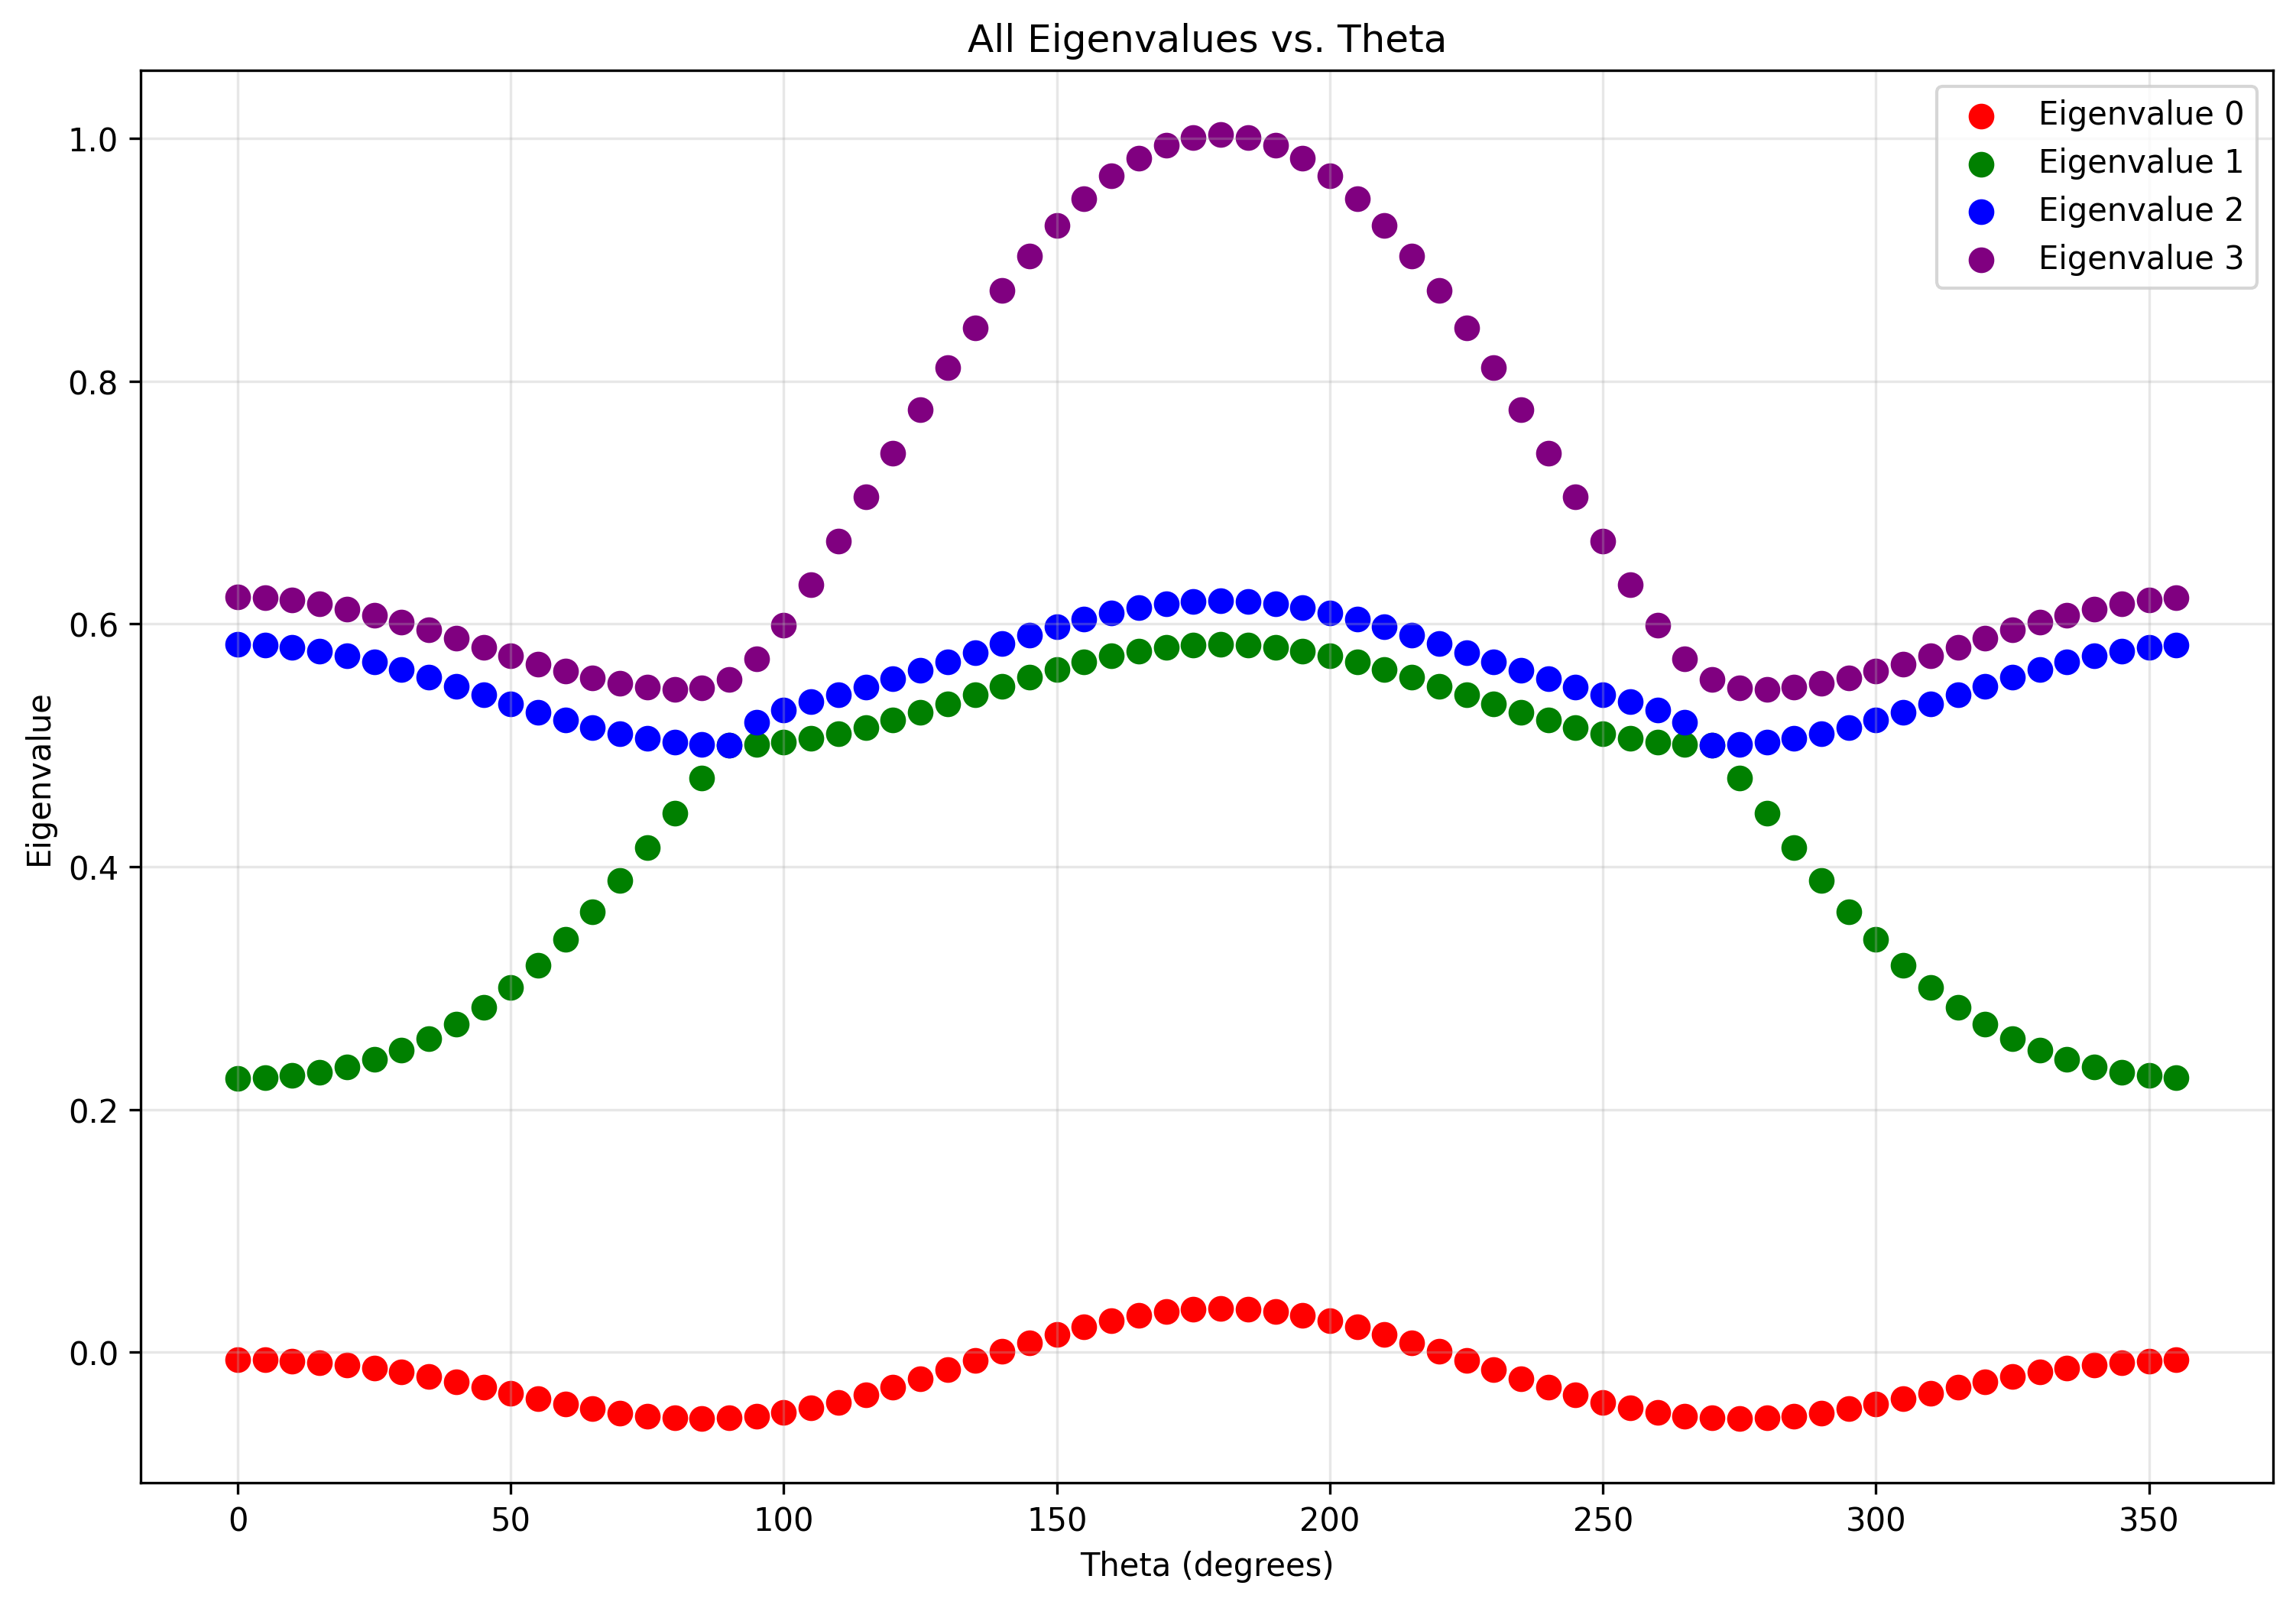
\includegraphics[width=0.8\textwidth]{../example_use/arrowhead_matrix/results/plots/all_eigenvalues_2d.png}
    \caption{All eigenvalues plotted against theta}
    \label{fig:all_eigenvalues_2d_gen}
\end{figure}

Individual plots for each eigenvalue are shown in Figures \ref{fig:eigenvalue_0_2d_gen} through \ref{fig:eigenvalue_3_2d_gen}.

\begin{figure}[H]
    \centering
    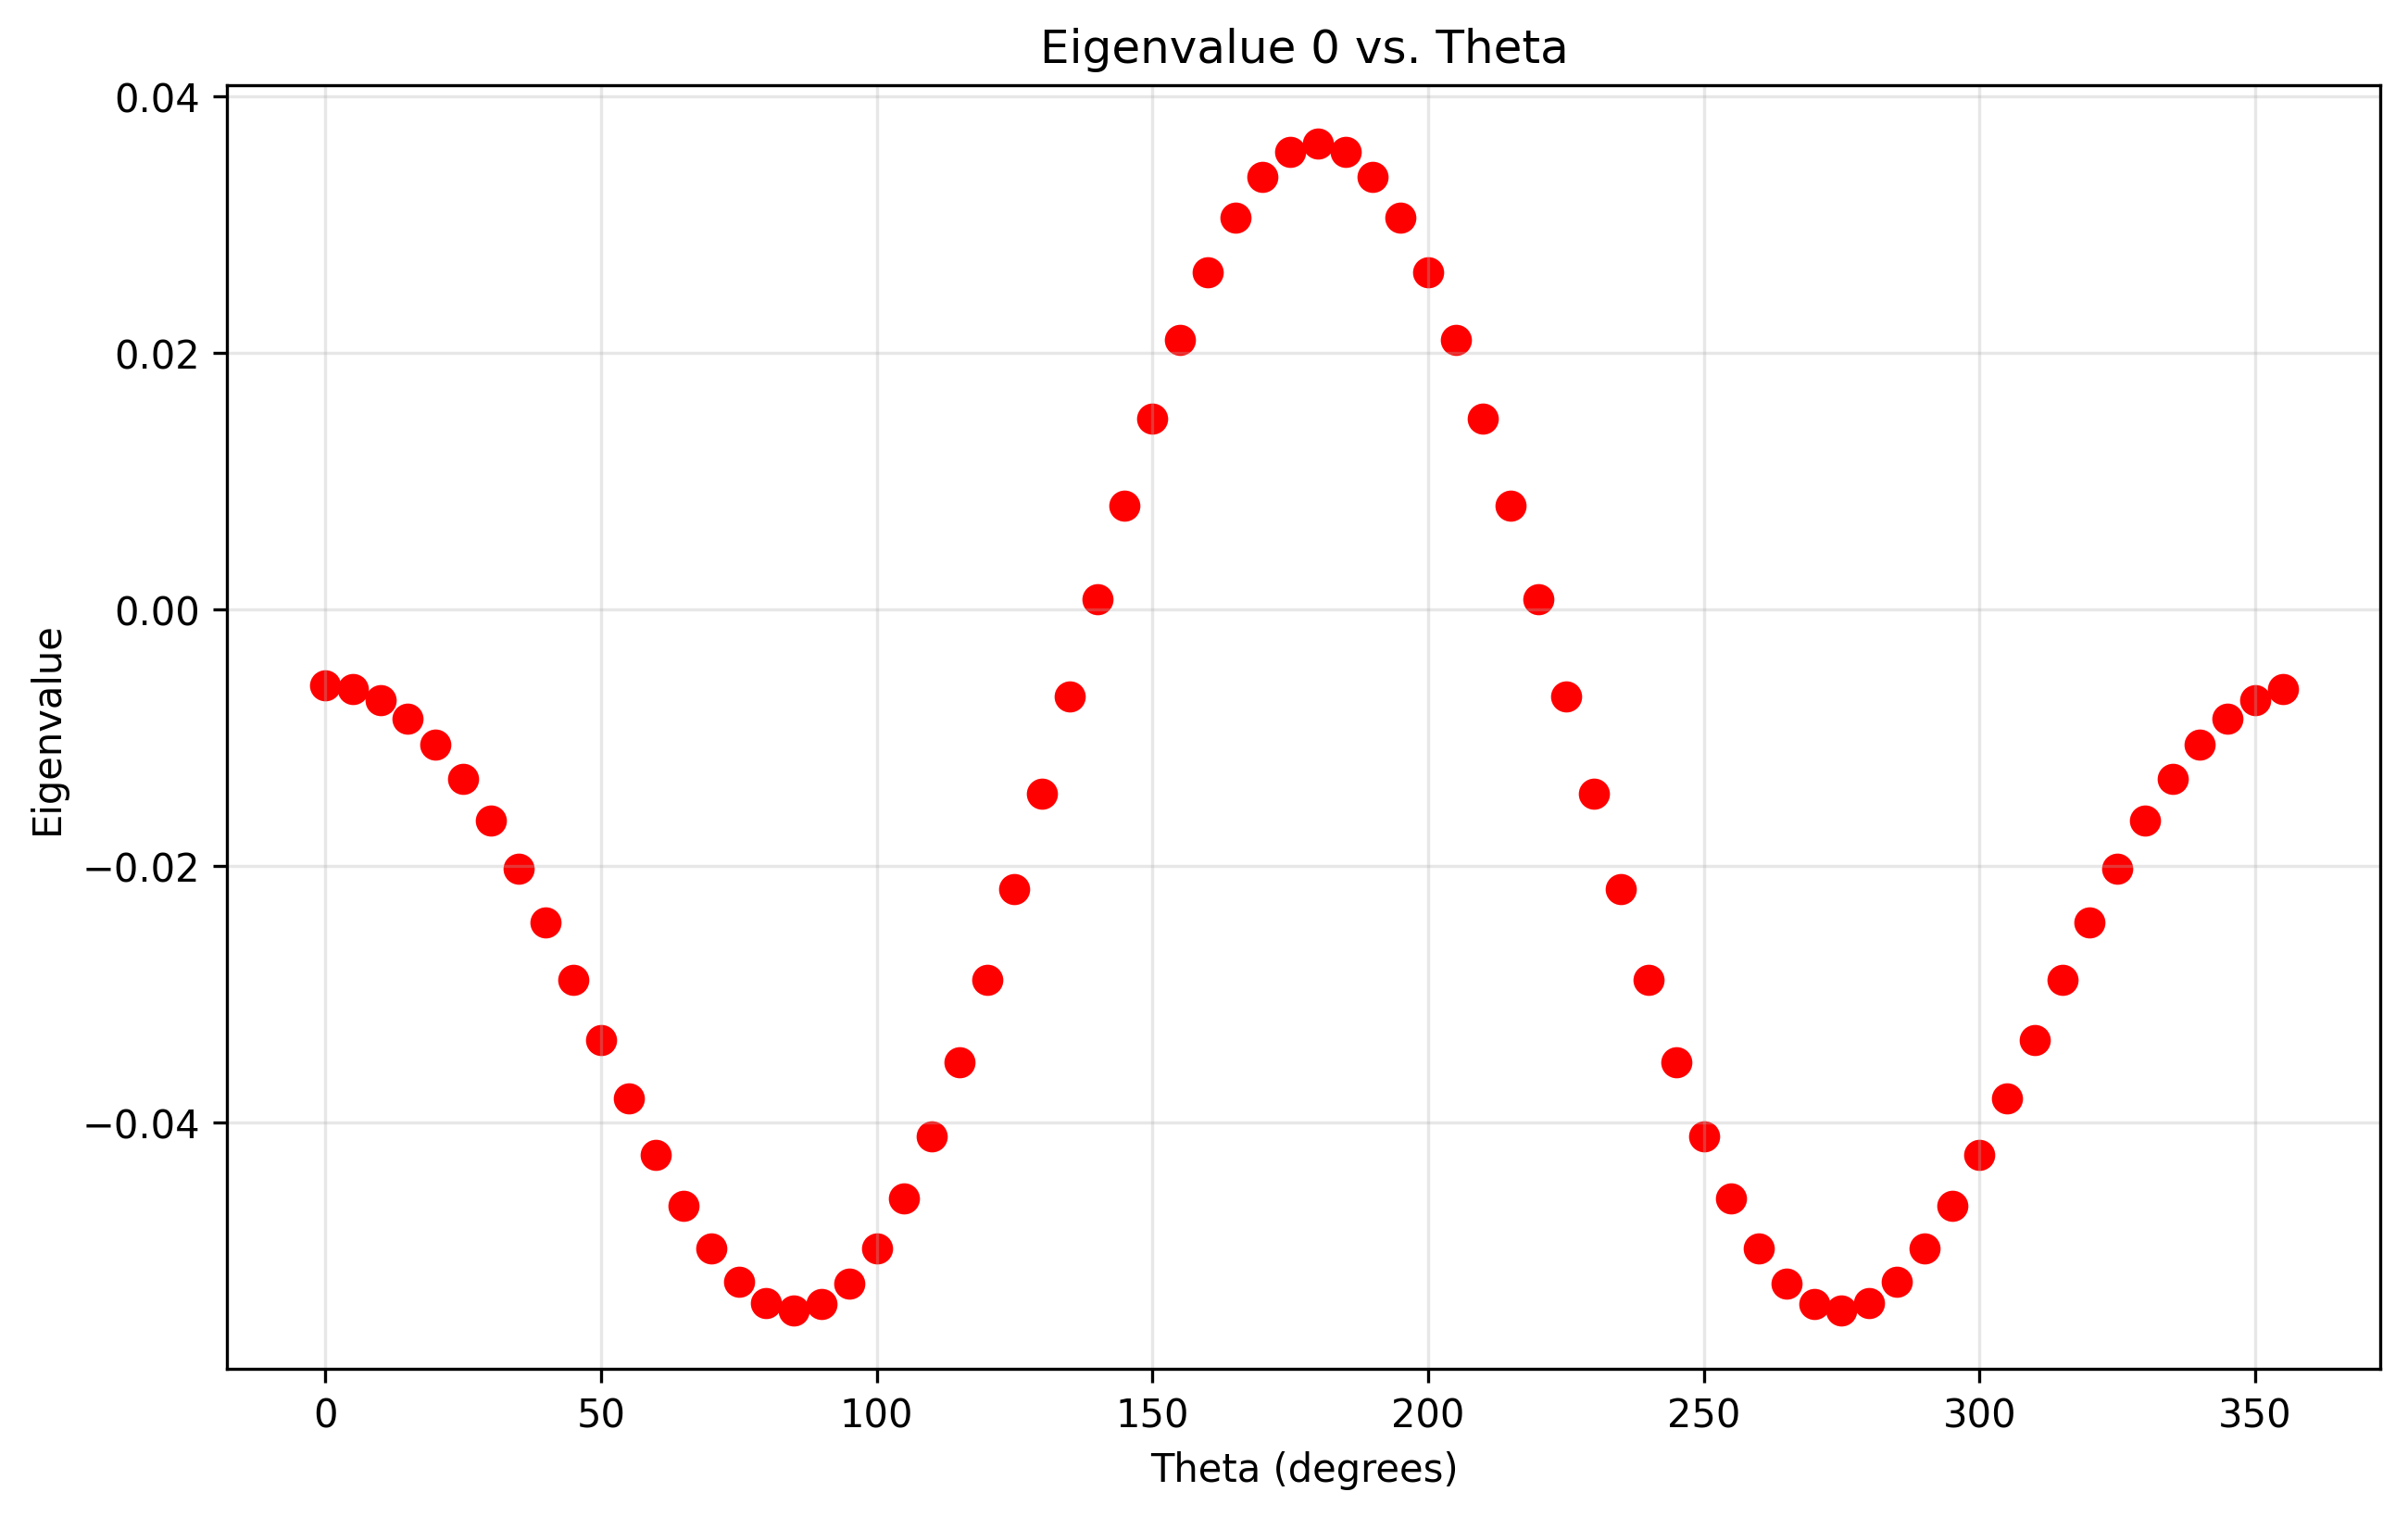
\includegraphics[width=0.8\textwidth]{../example_use/arrowhead_matrix/results/plots/eigenvalue_0_2d.png}
    \caption{First eigenvalue plotted against theta}
    \label{fig:eigenvalue_0_2d_gen}
\end{figure}

\begin{figure}[H]
    \centering
    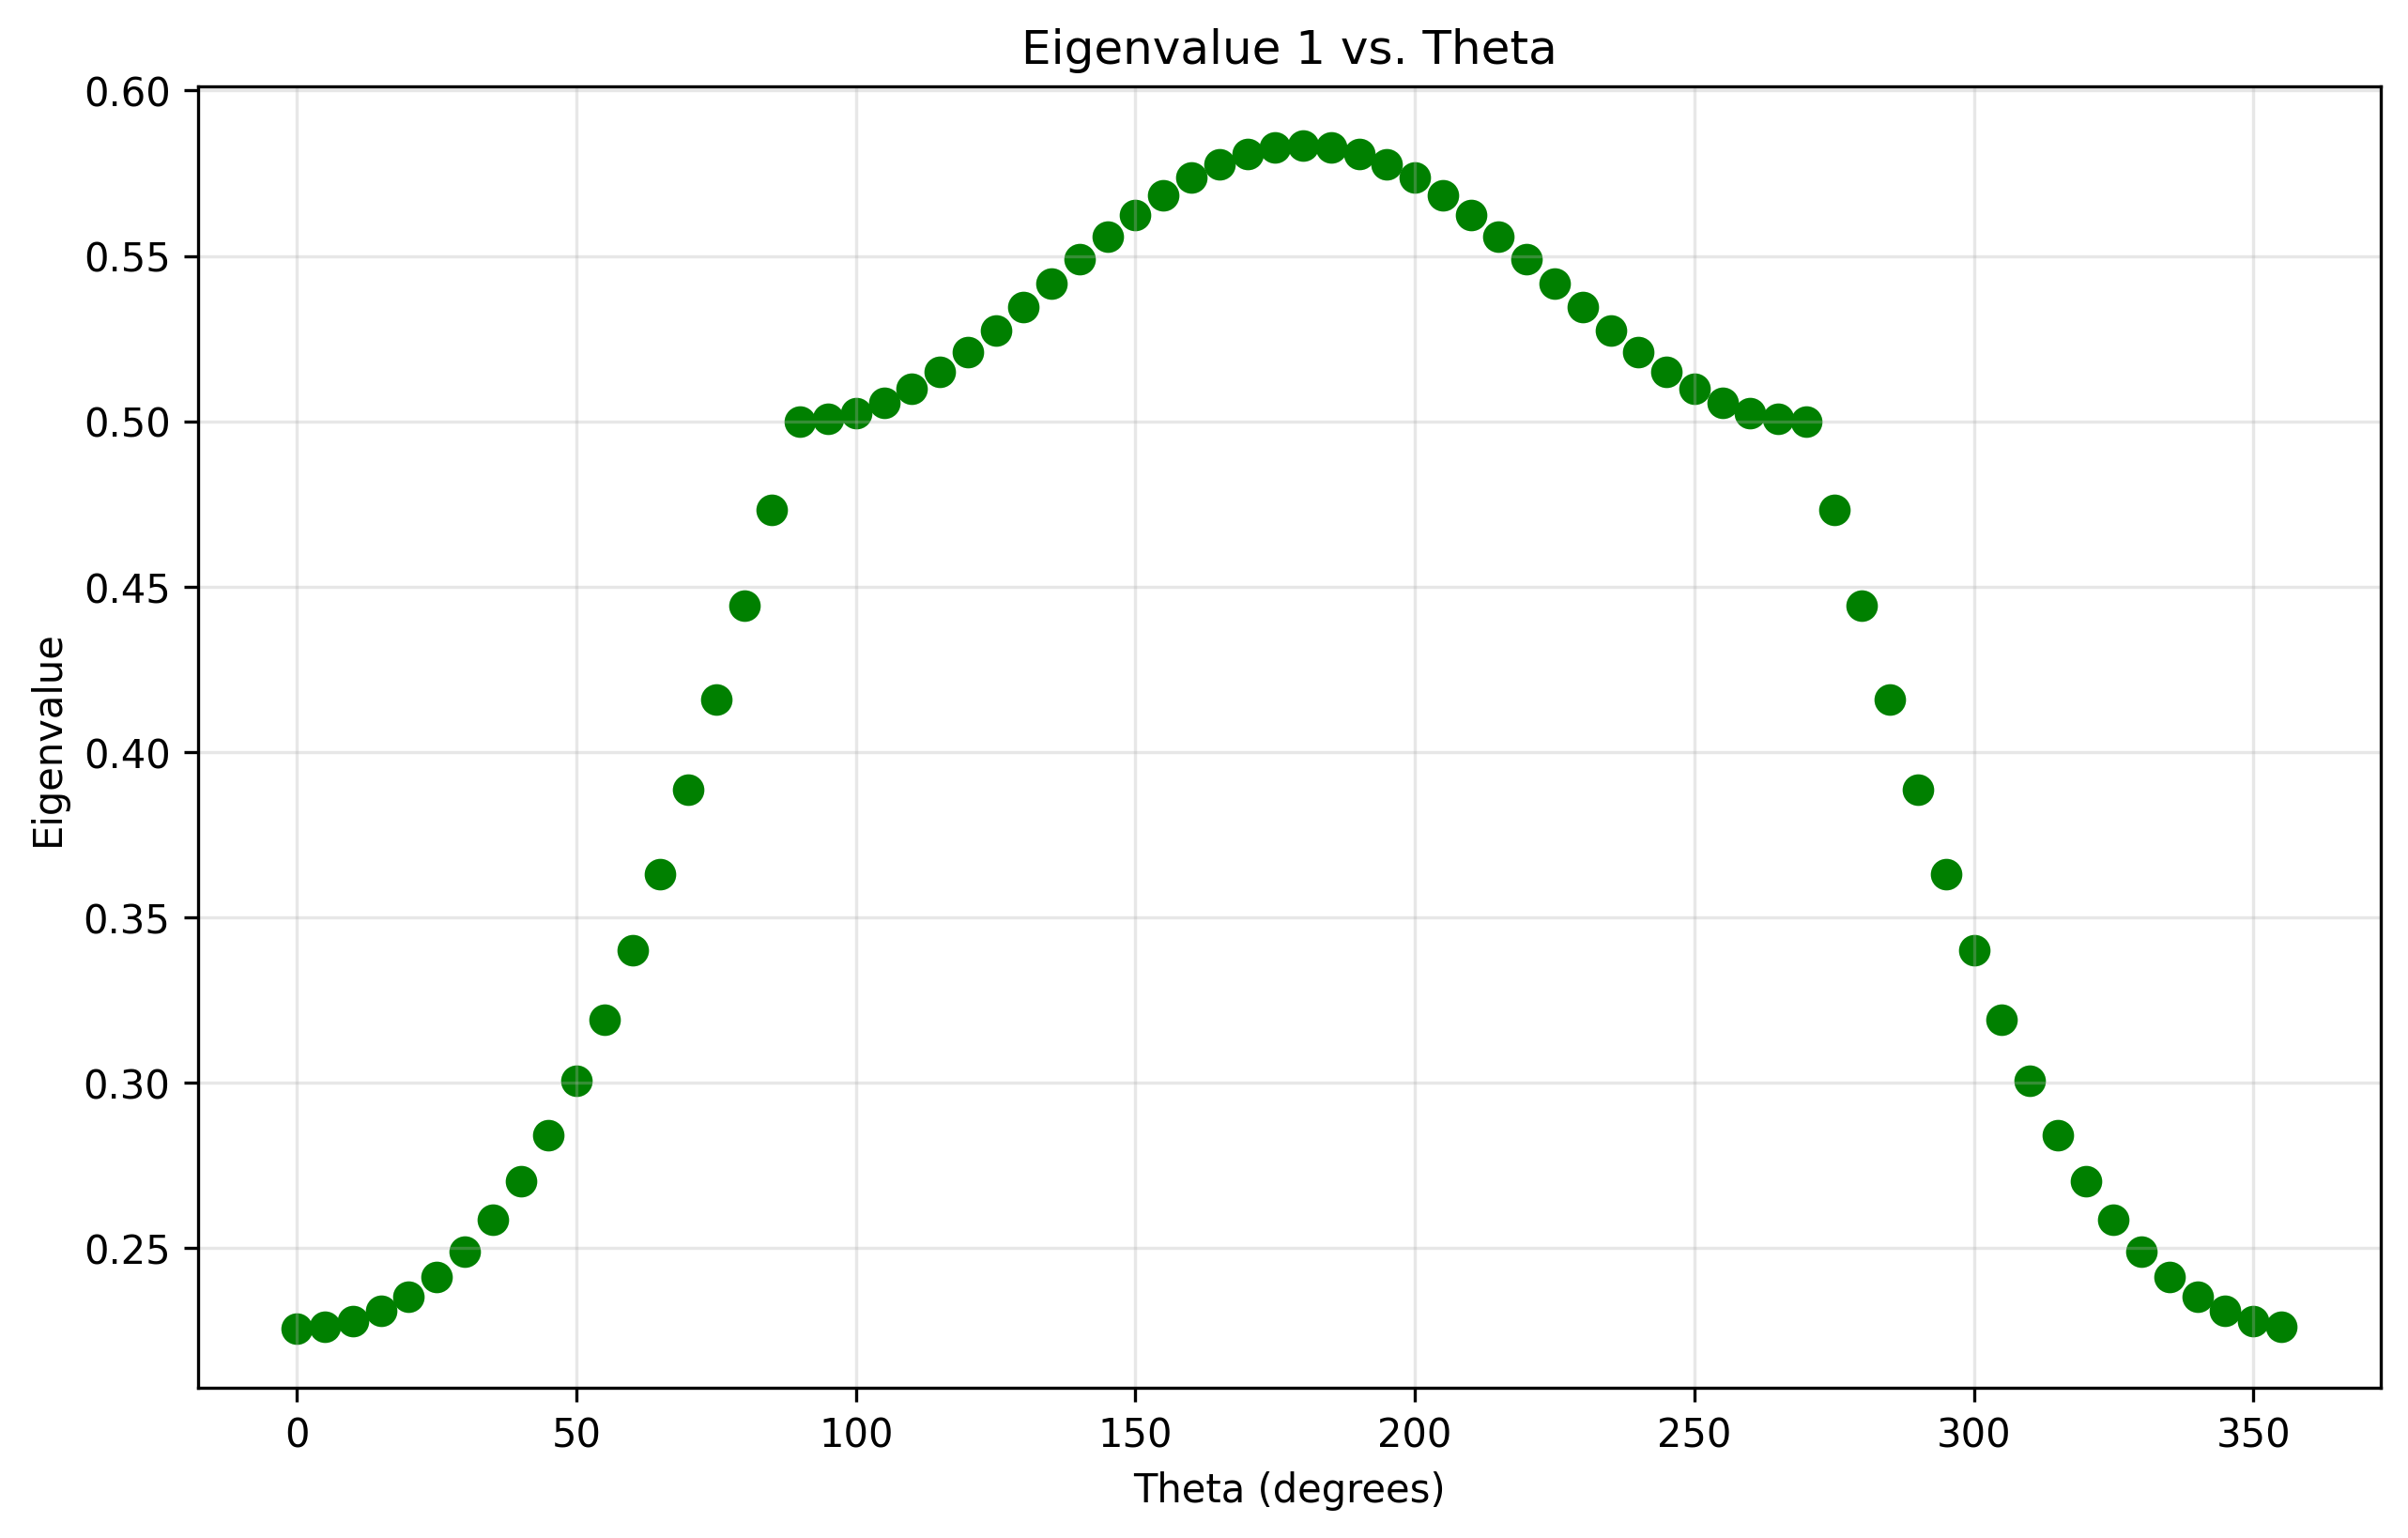
\includegraphics[width=0.8\textwidth]{../example_use/arrowhead_matrix/results/plots/eigenvalue_1_2d.png}
    \caption{Second eigenvalue plotted against theta}
    \label{fig:eigenvalue_1_2d_gen}
\end{figure}

\begin{figure}[H]
    \centering
    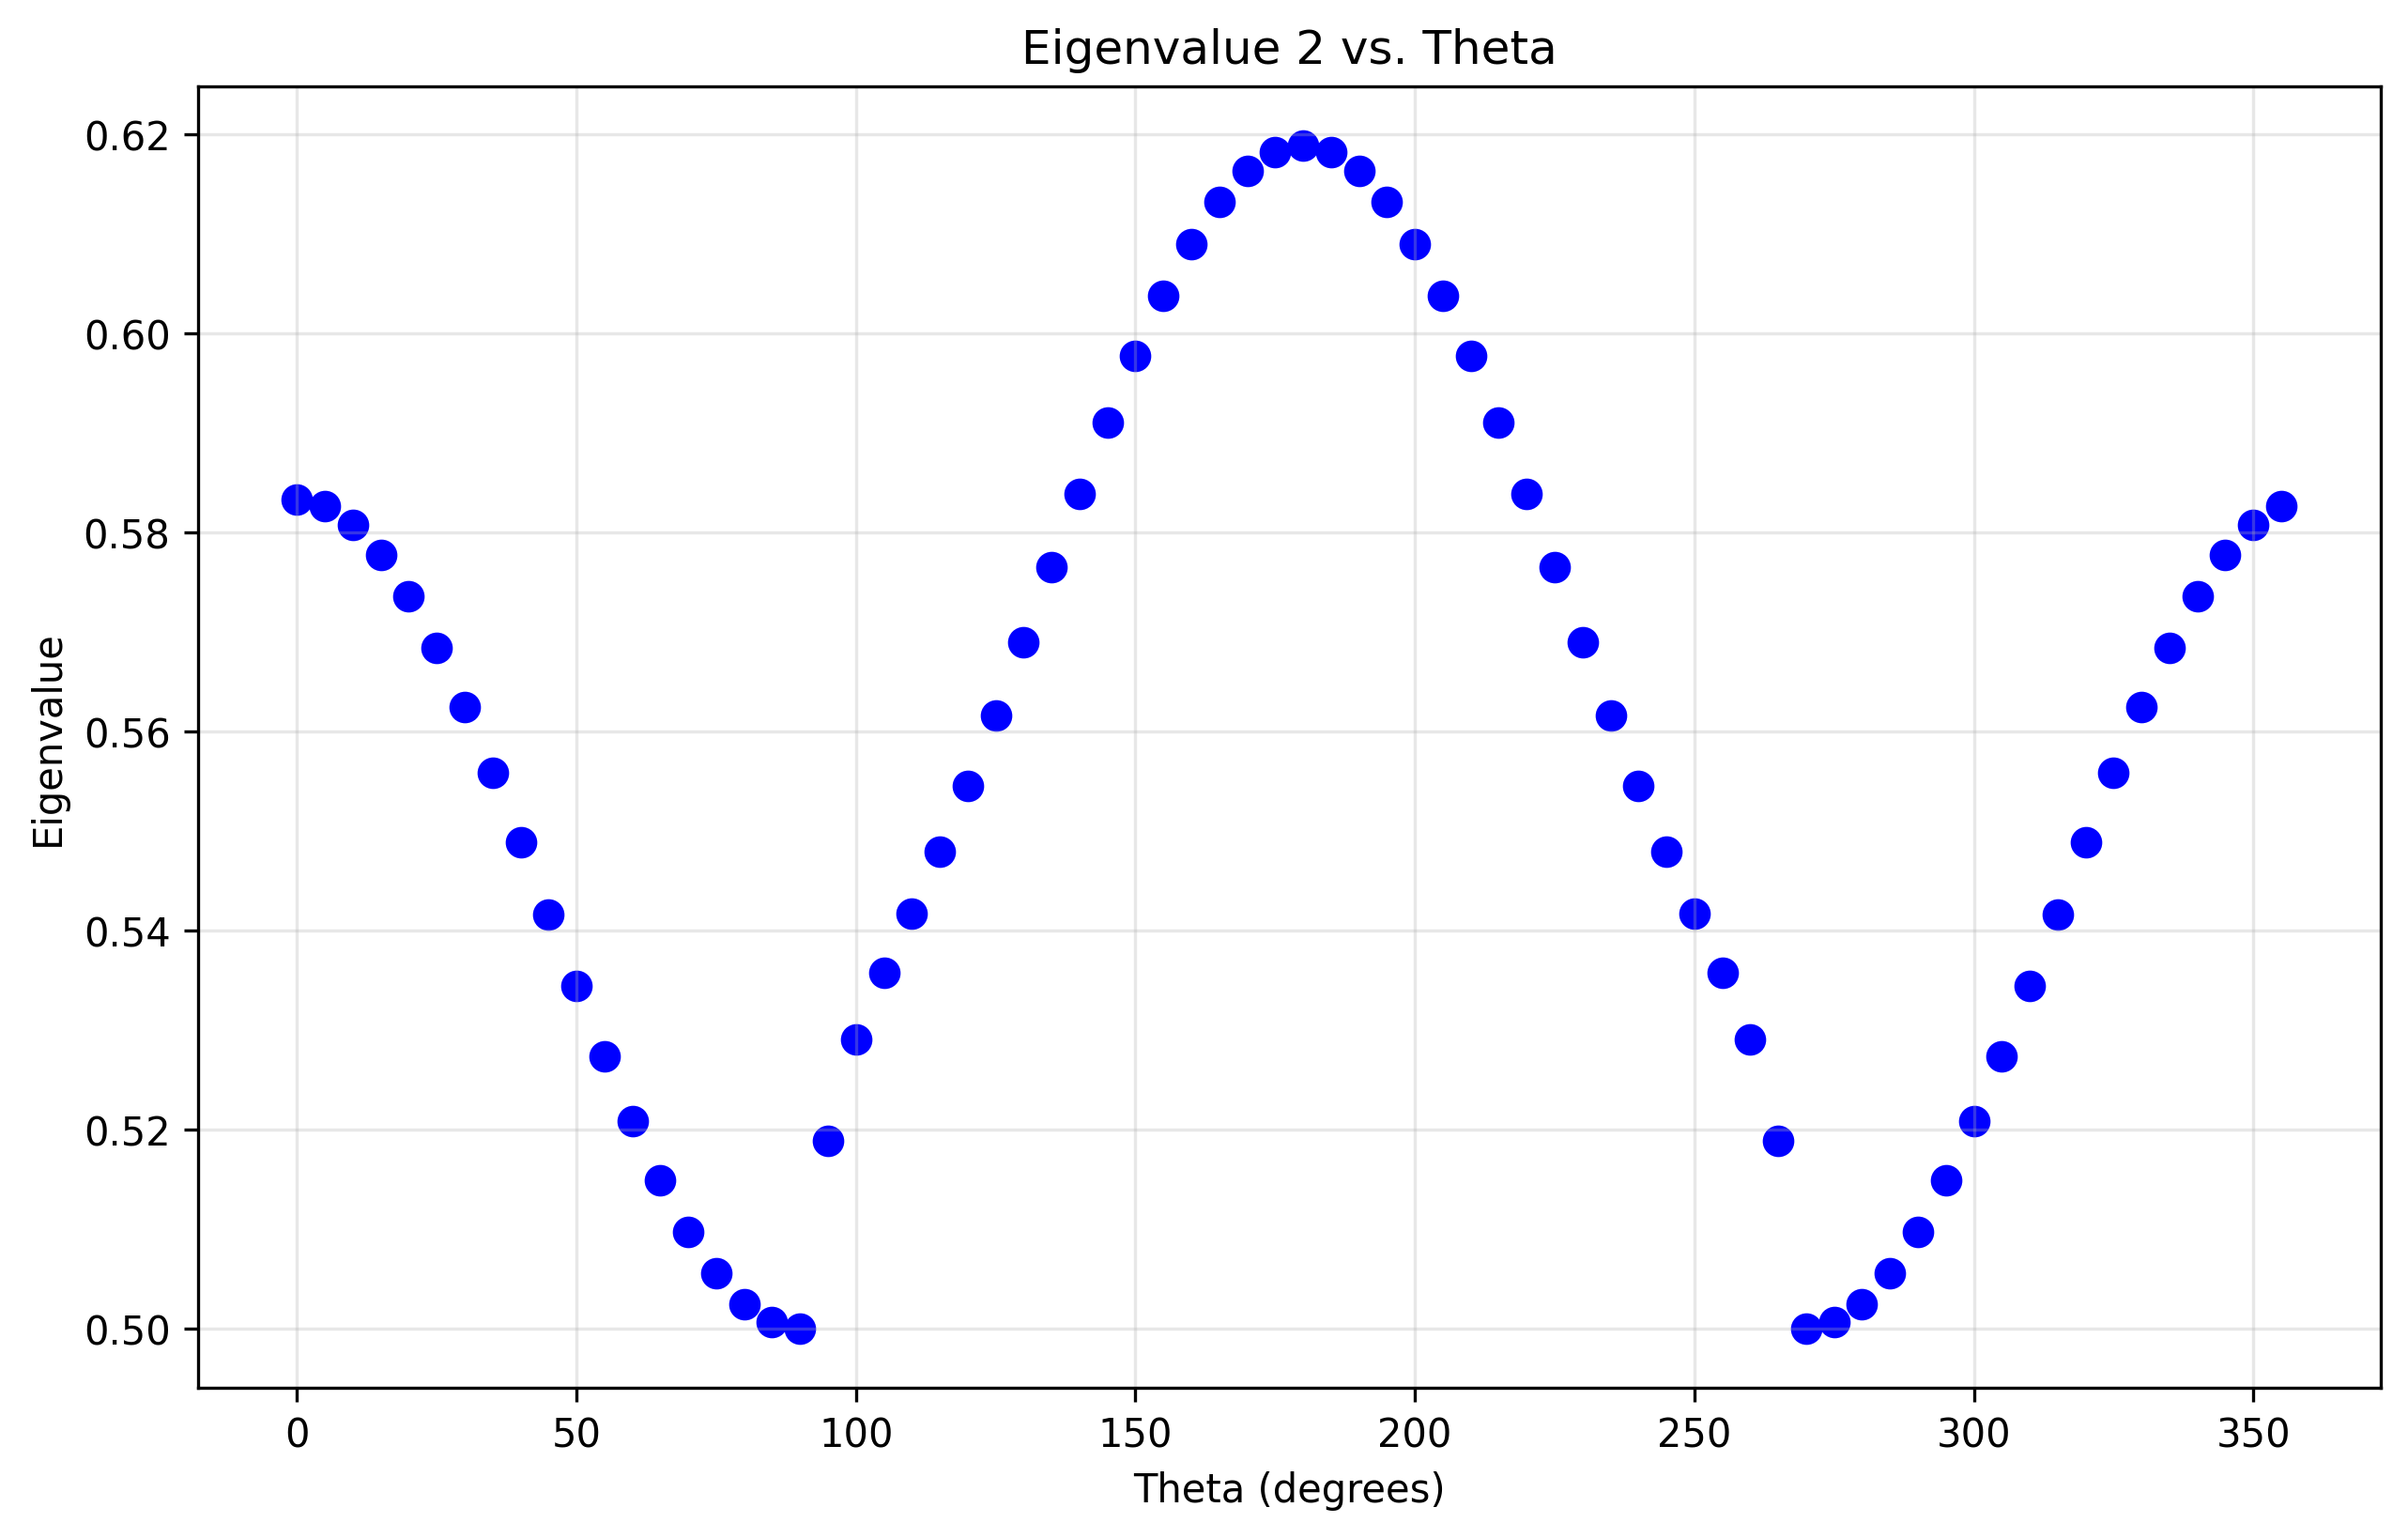
\includegraphics[width=0.8\textwidth]{../example_use/arrowhead_matrix/results/plots/eigenvalue_2_2d.png}
    \caption{Third eigenvalue plotted against theta}
    \label{fig:eigenvalue_2_2d_gen}
\end{figure}

\begin{figure}[H]
    \centering
    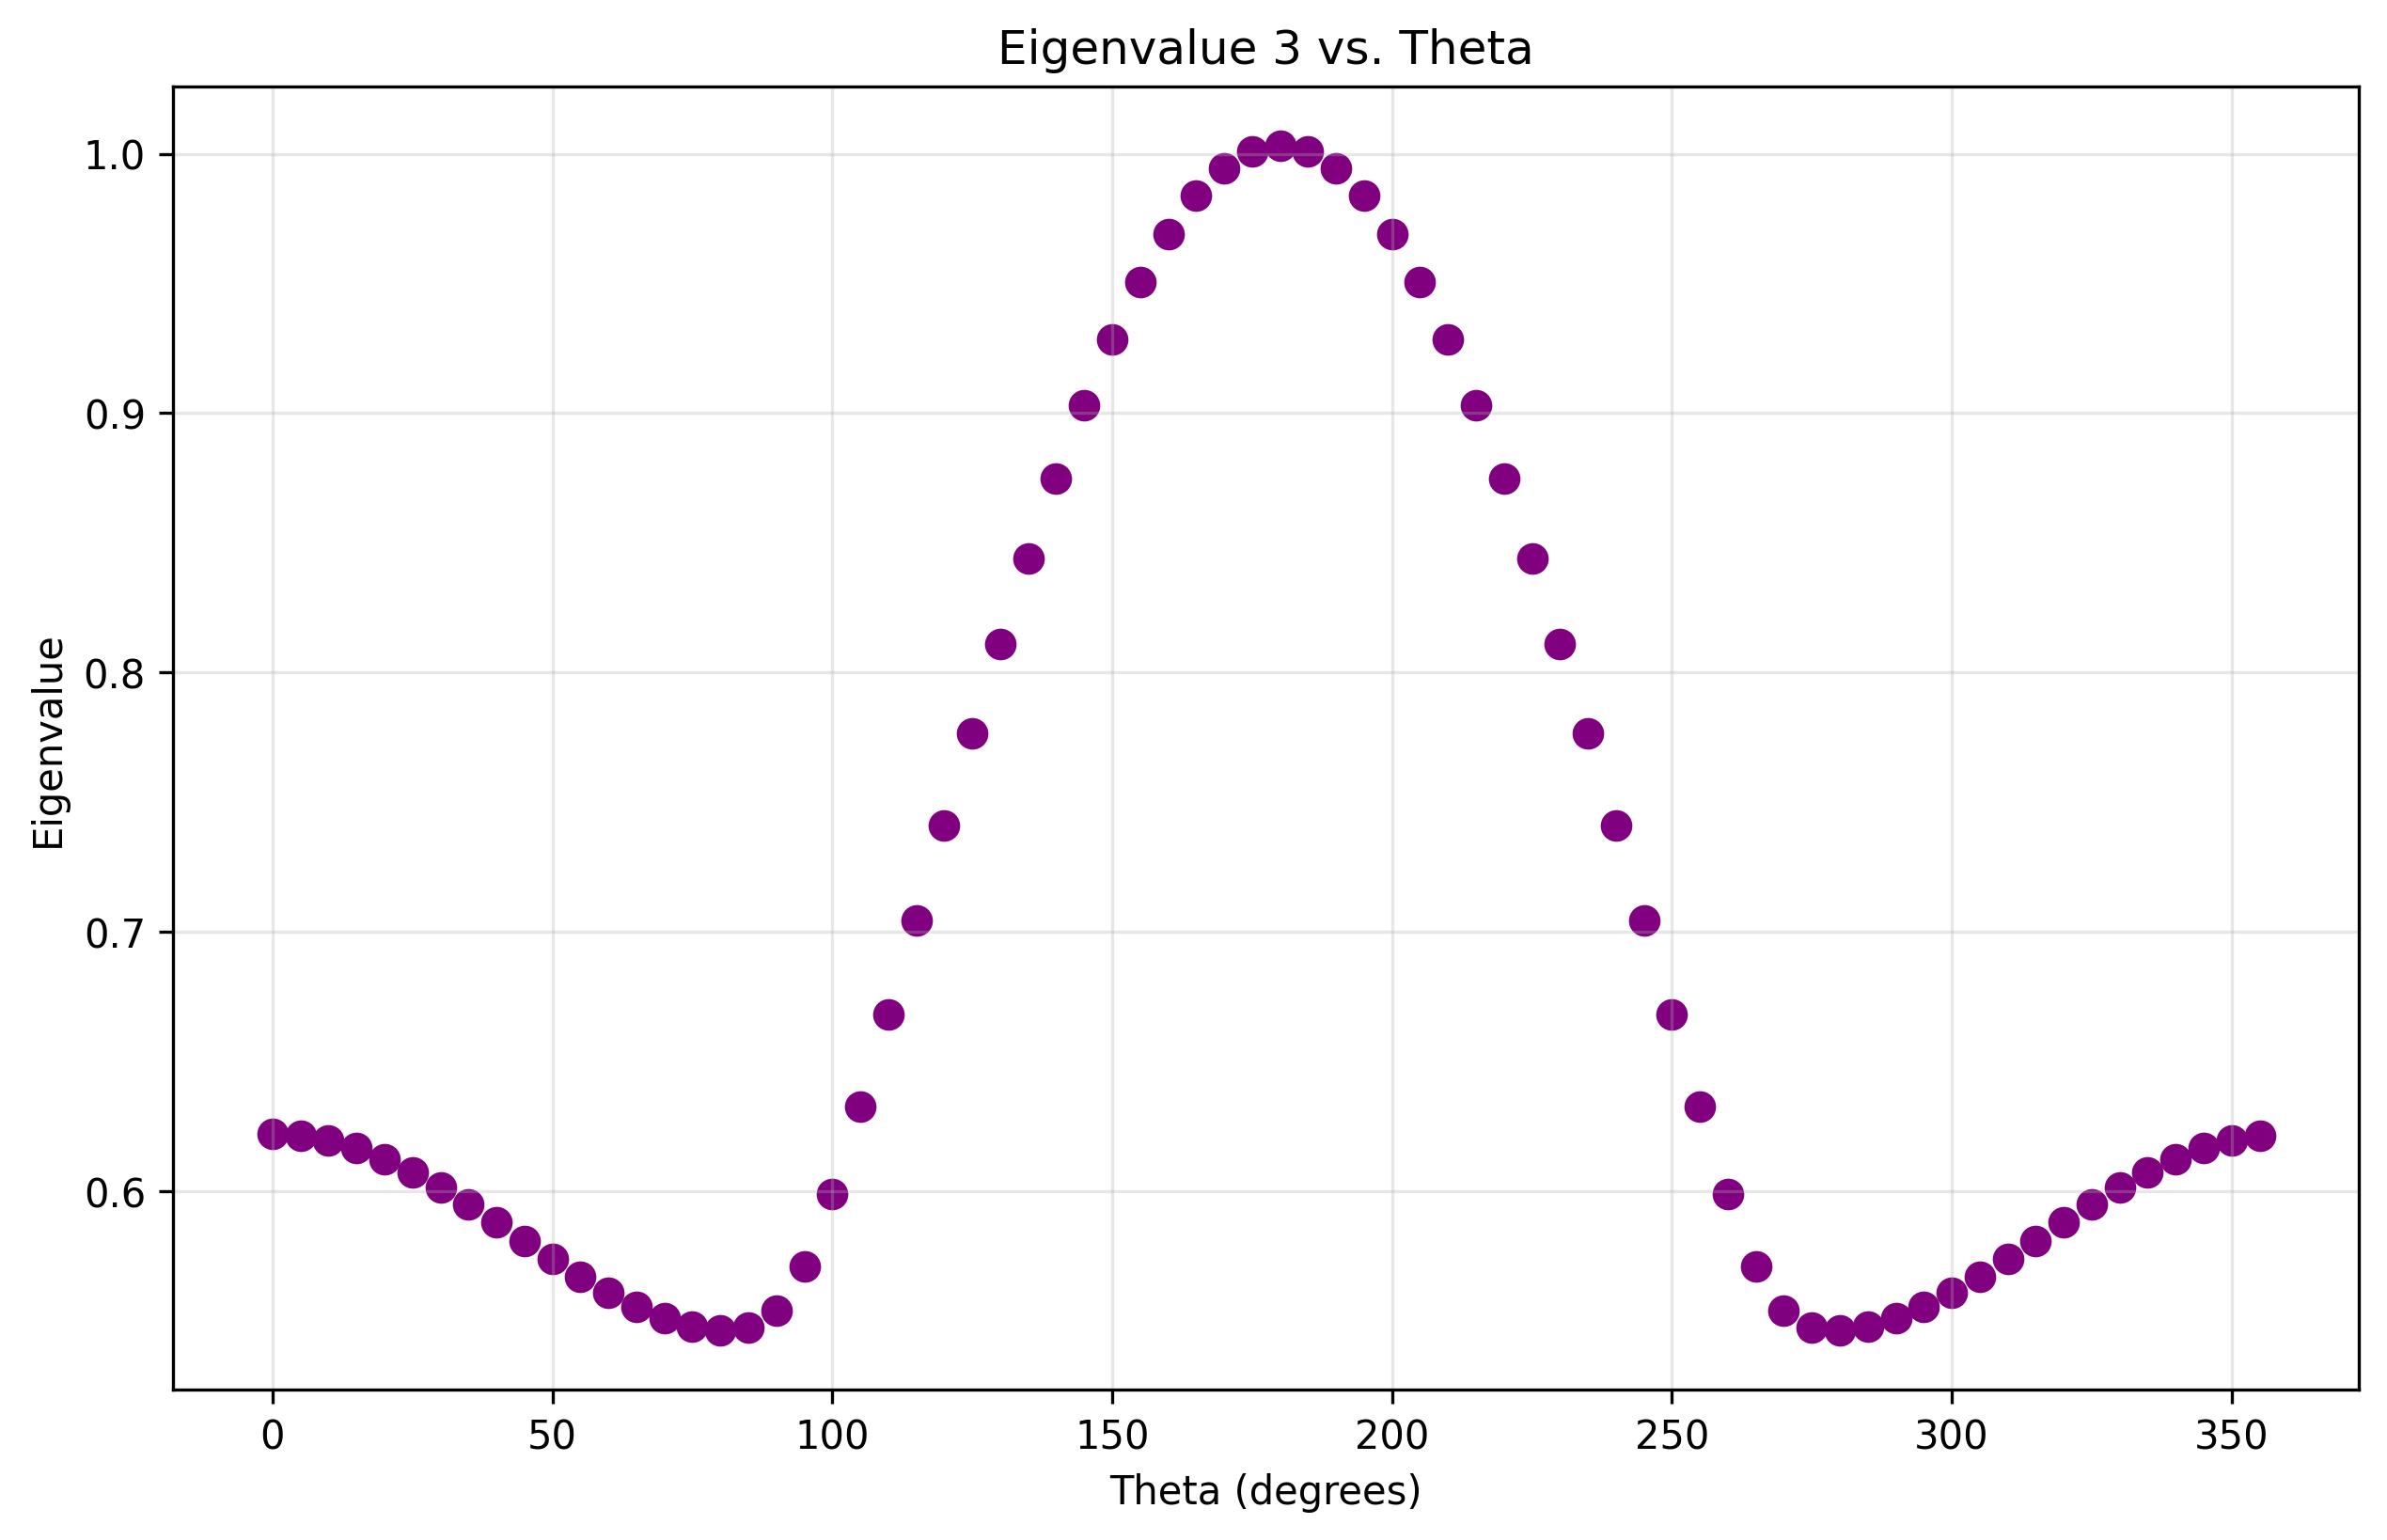
\includegraphics[width=0.8\textwidth]{../example_use/arrowhead_matrix/results/plots/eigenvalue_3_2d.png}
    \caption{Fourth eigenvalue plotted against theta}
    \label{fig:eigenvalue_3_2d_gen}
\end{figure}

\subsubsection{Eigenvector Visualization}

Figure \ref{fig:eigenvectors_no_labels_gen} shows the endpoints of all eigenvectors for different values of $\theta$ without labels for clarity.

\begin{figure}[H]
    \centering
    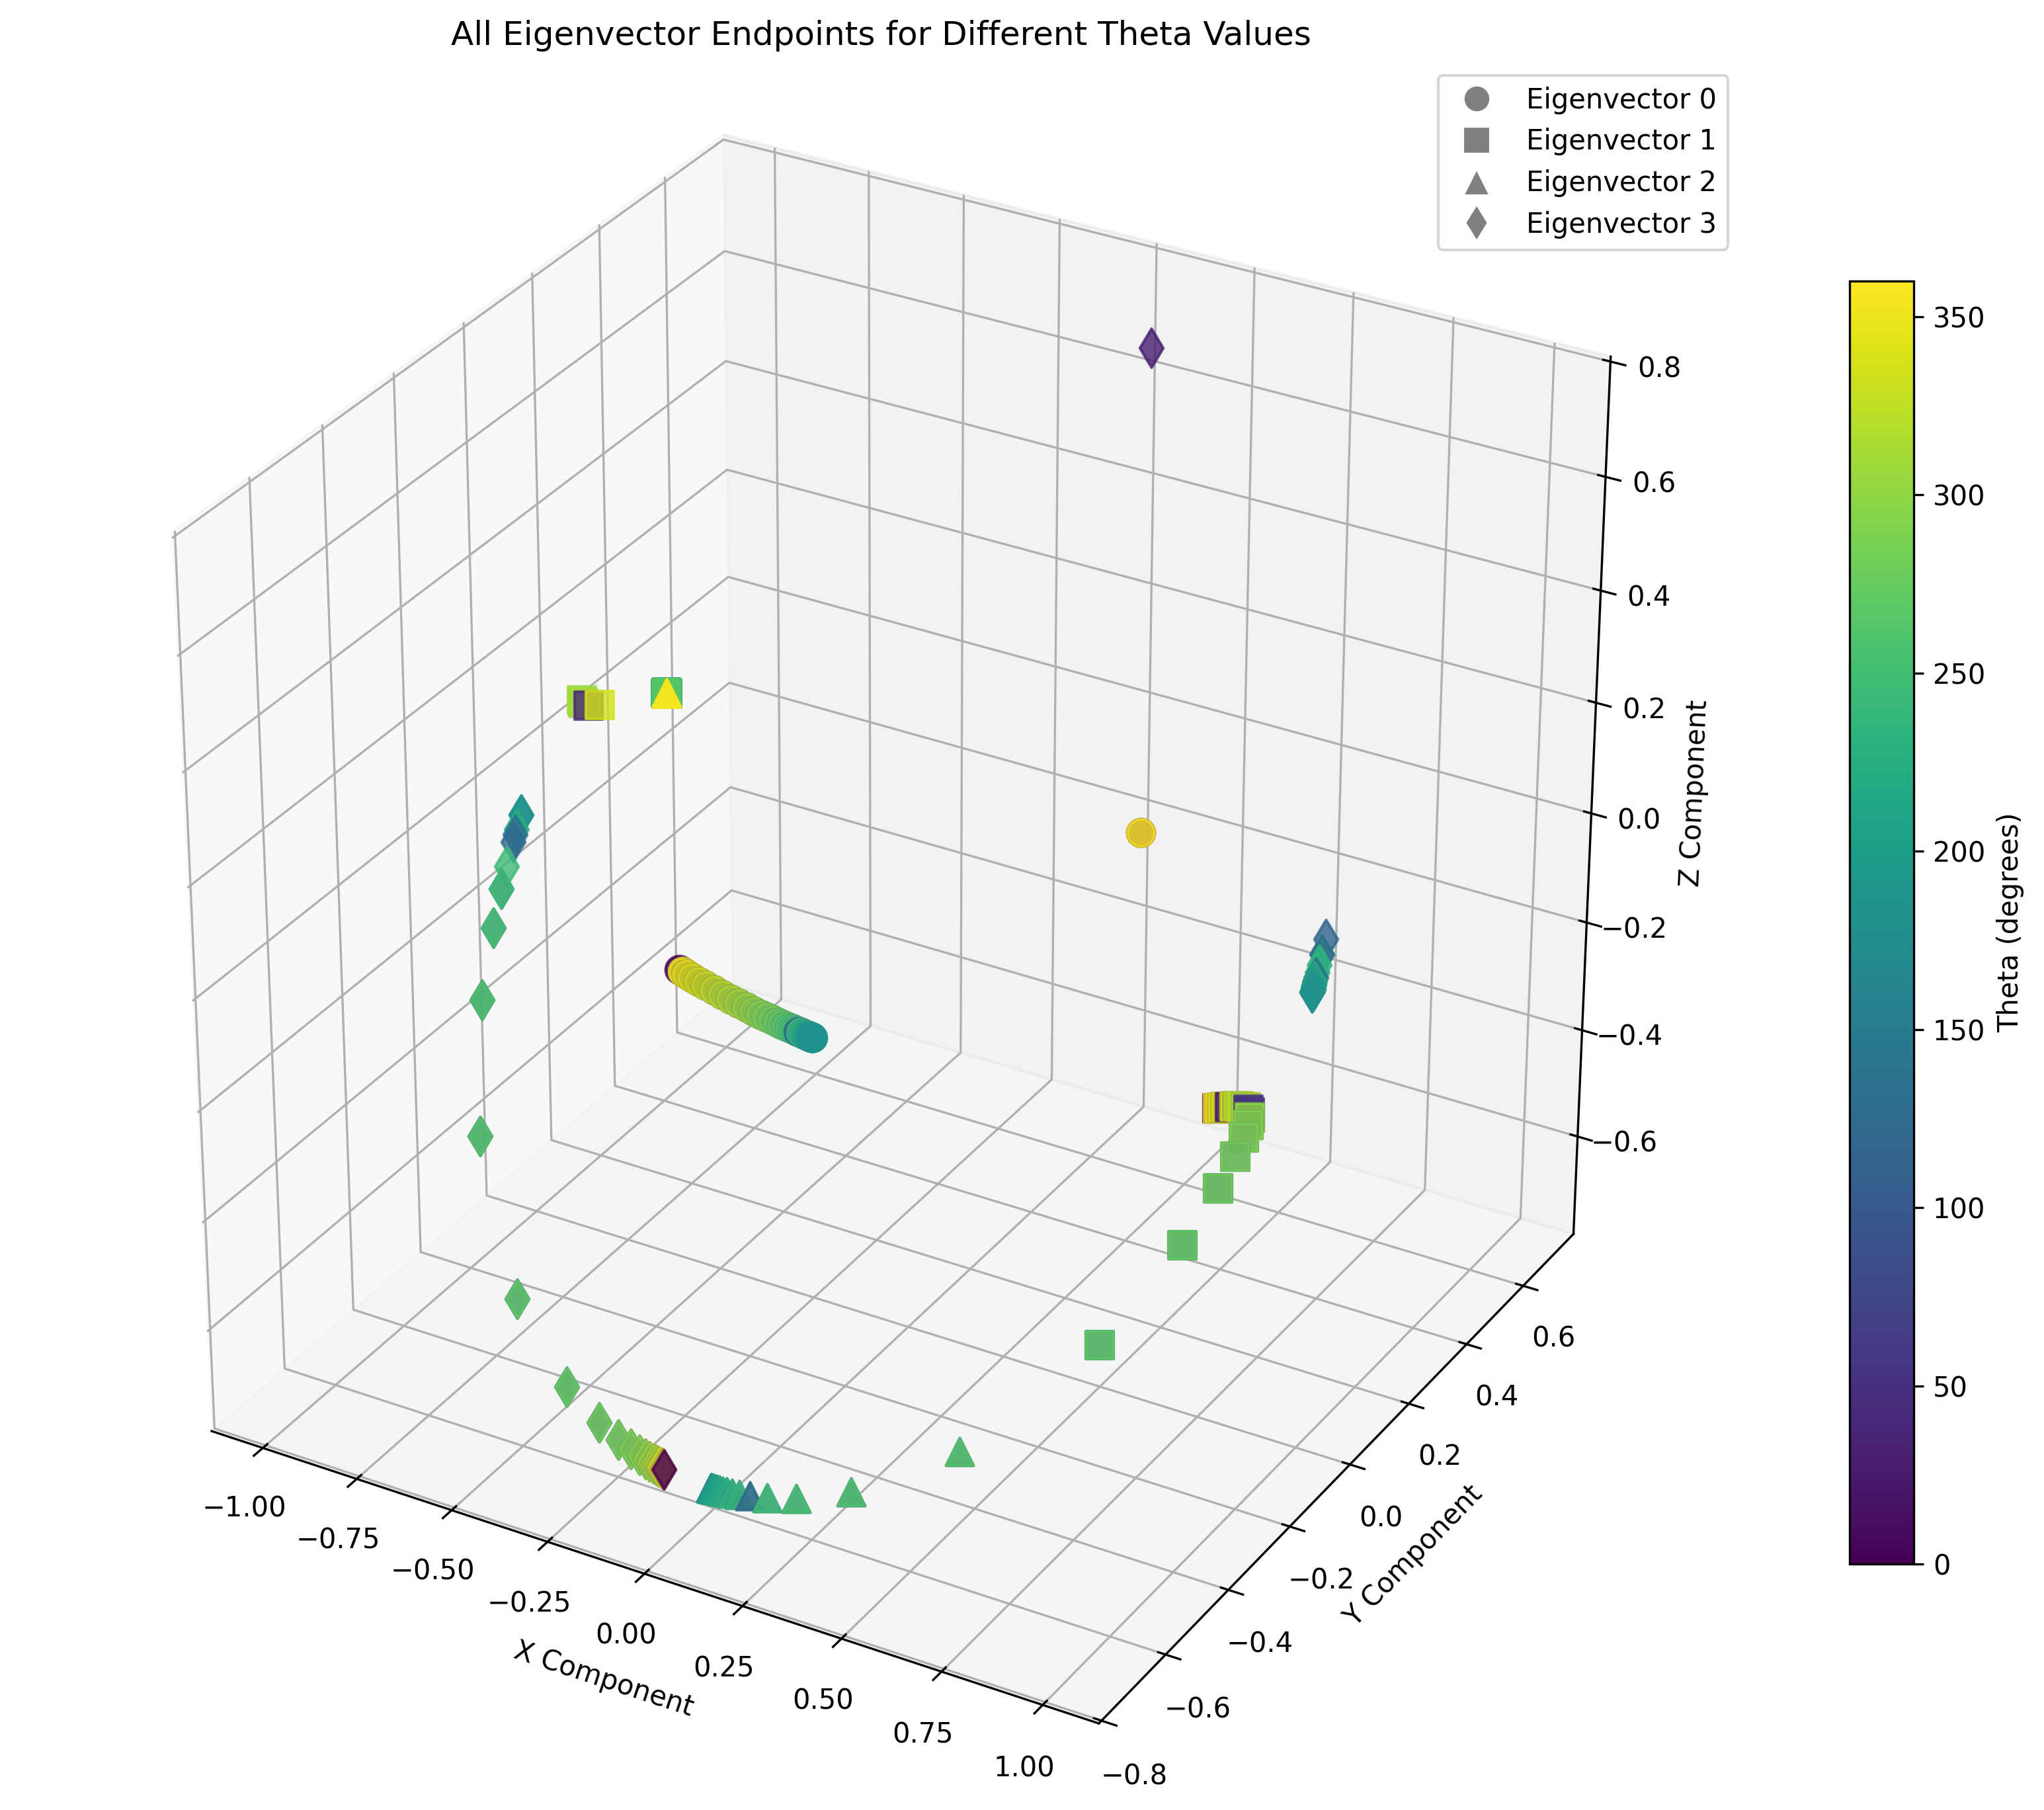
\includegraphics[width=0.8\textwidth]{../example_use/arrowhead_matrix/results/plots/eigenvectors_no_labels.png}
    \caption{3D visualization of all eigenvector endpoints (without labels)}
    \label{fig:eigenvectors_no_labels_gen}
\end{figure}

Individual plots for each eigenvector are shown in Figures \ref{fig:eigenvector_0_no_labels_gen} through \ref{fig:eigenvector_3_no_labels_gen}.

\begin{figure}[H]
    \centering
    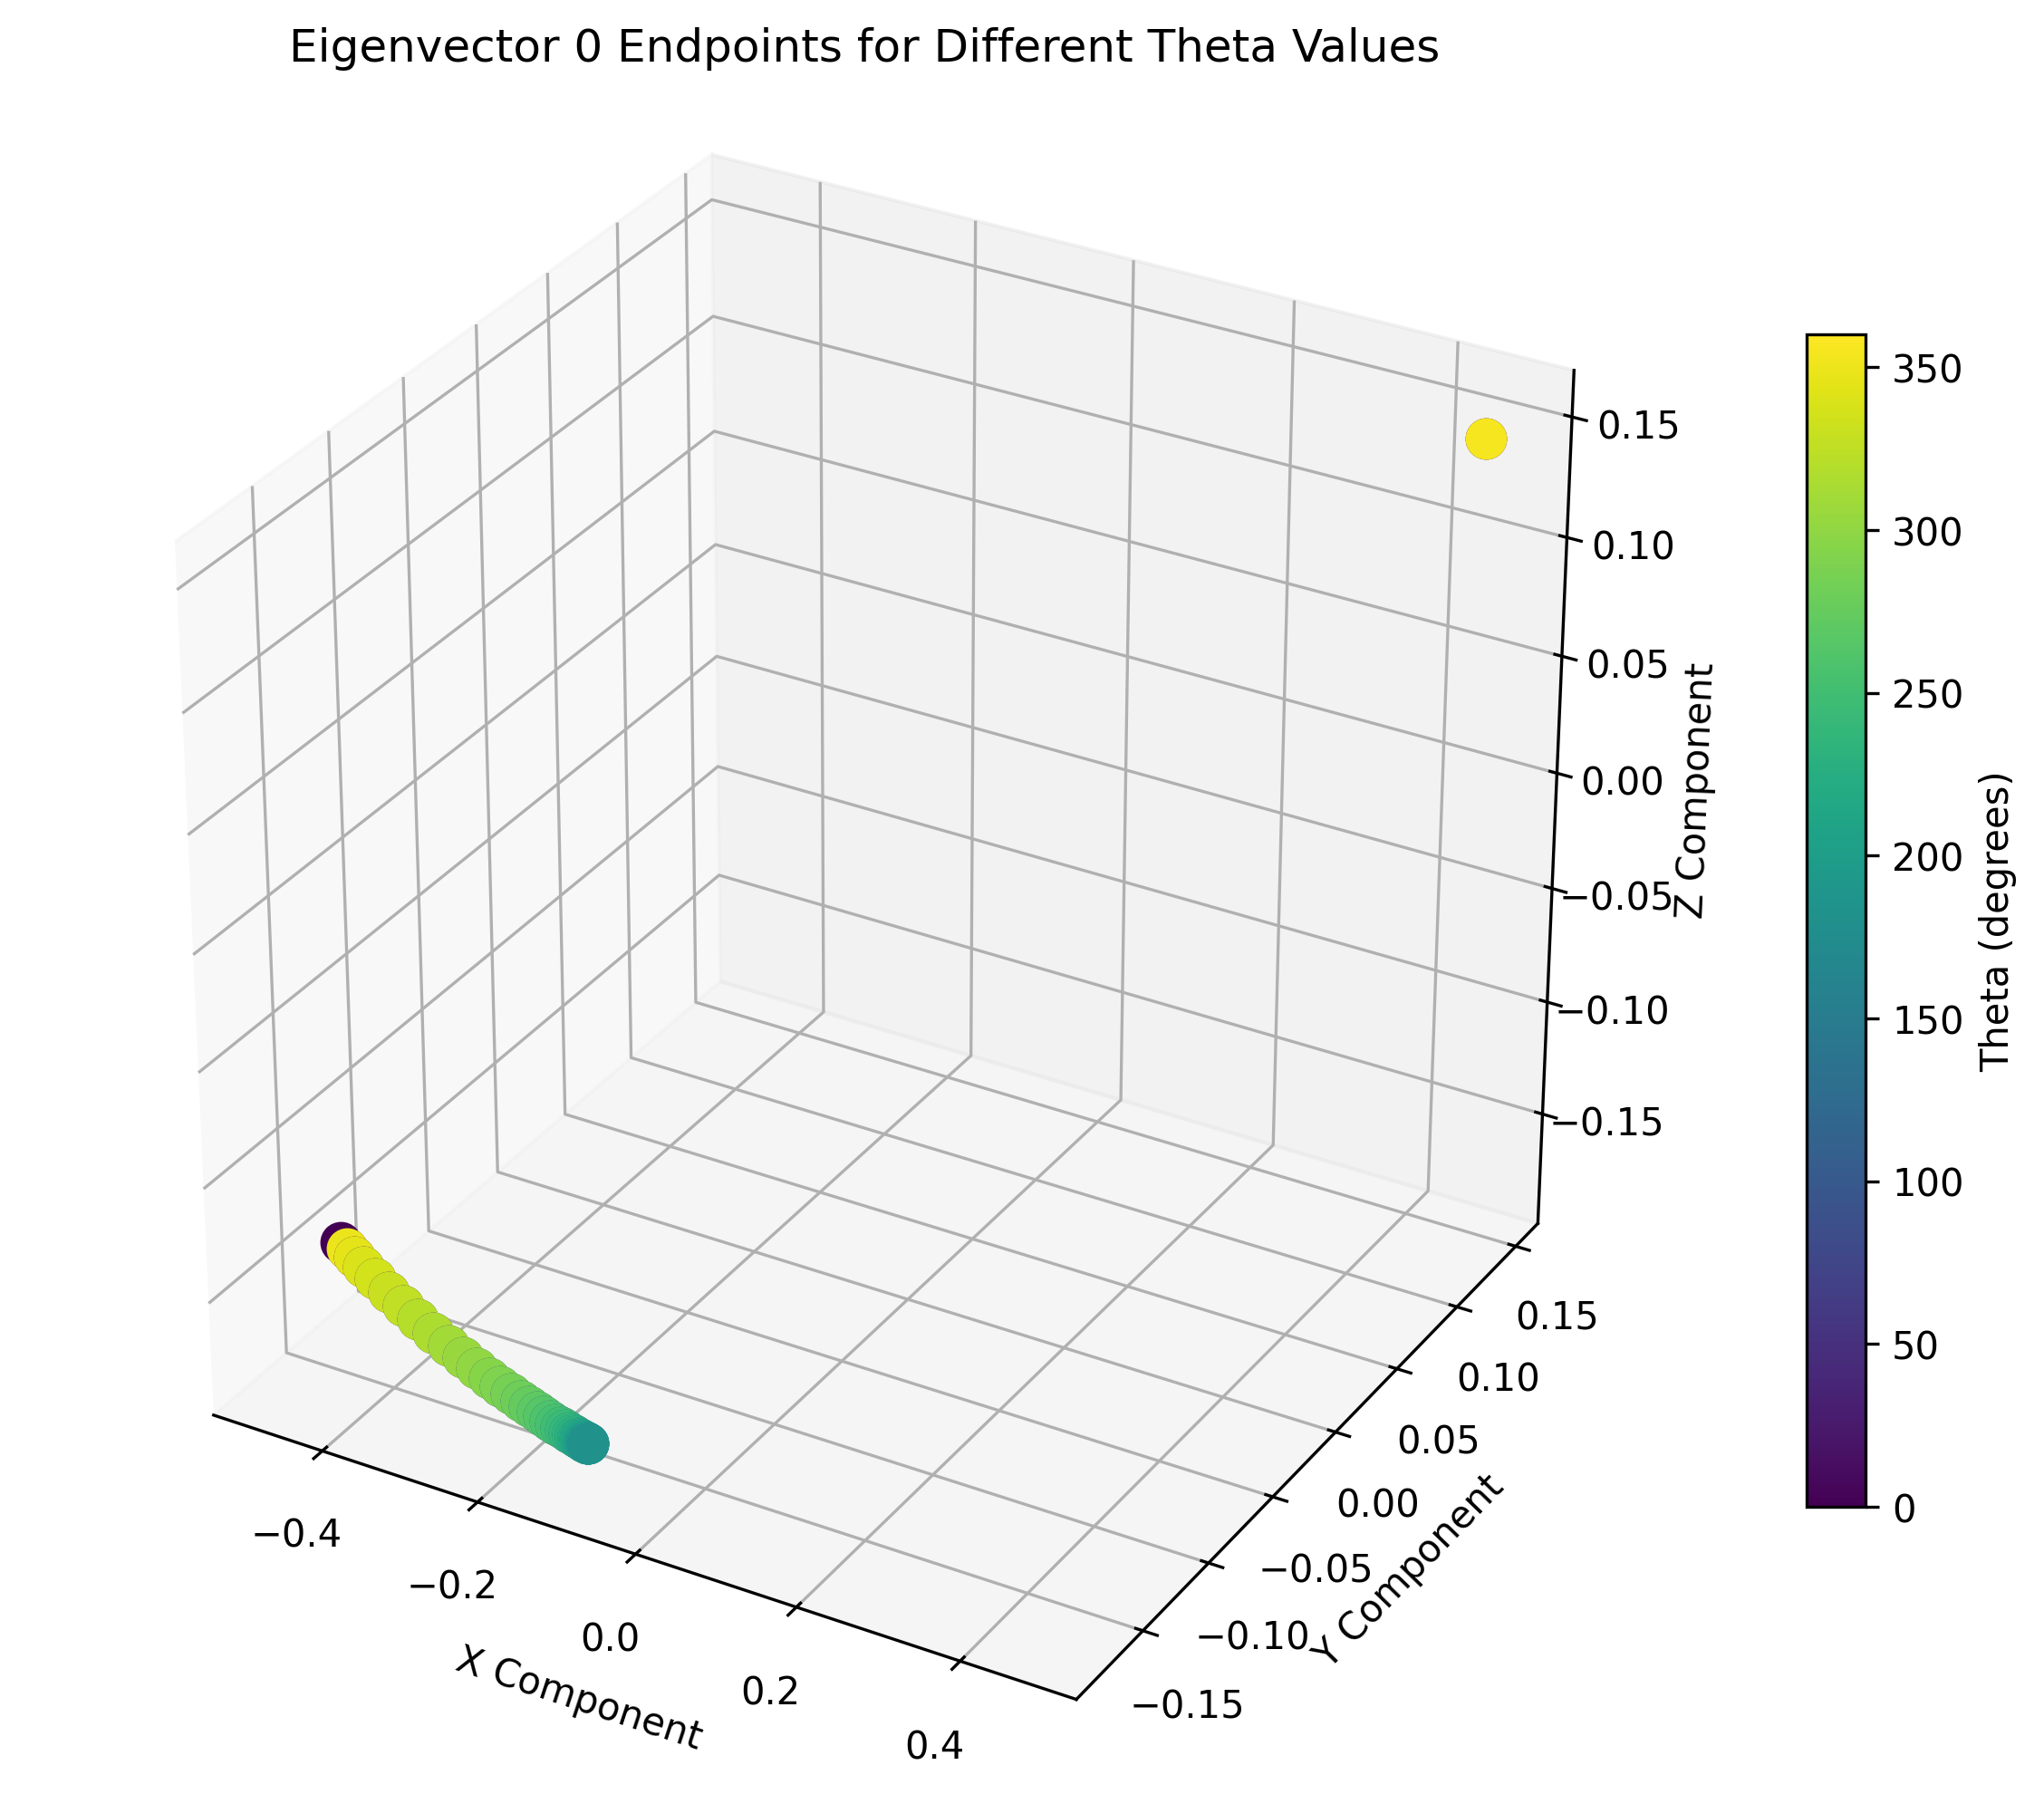
\includegraphics[width=0.8\textwidth]{../example_use/arrowhead_matrix/results/plots/eigenvector_0_no_labels.png}
    \caption{First eigenvector endpoints for different $\theta$ values}
    \label{fig:eigenvector_0_no_labels_gen}
\end{figure}

\begin{figure}[H]
    \centering
    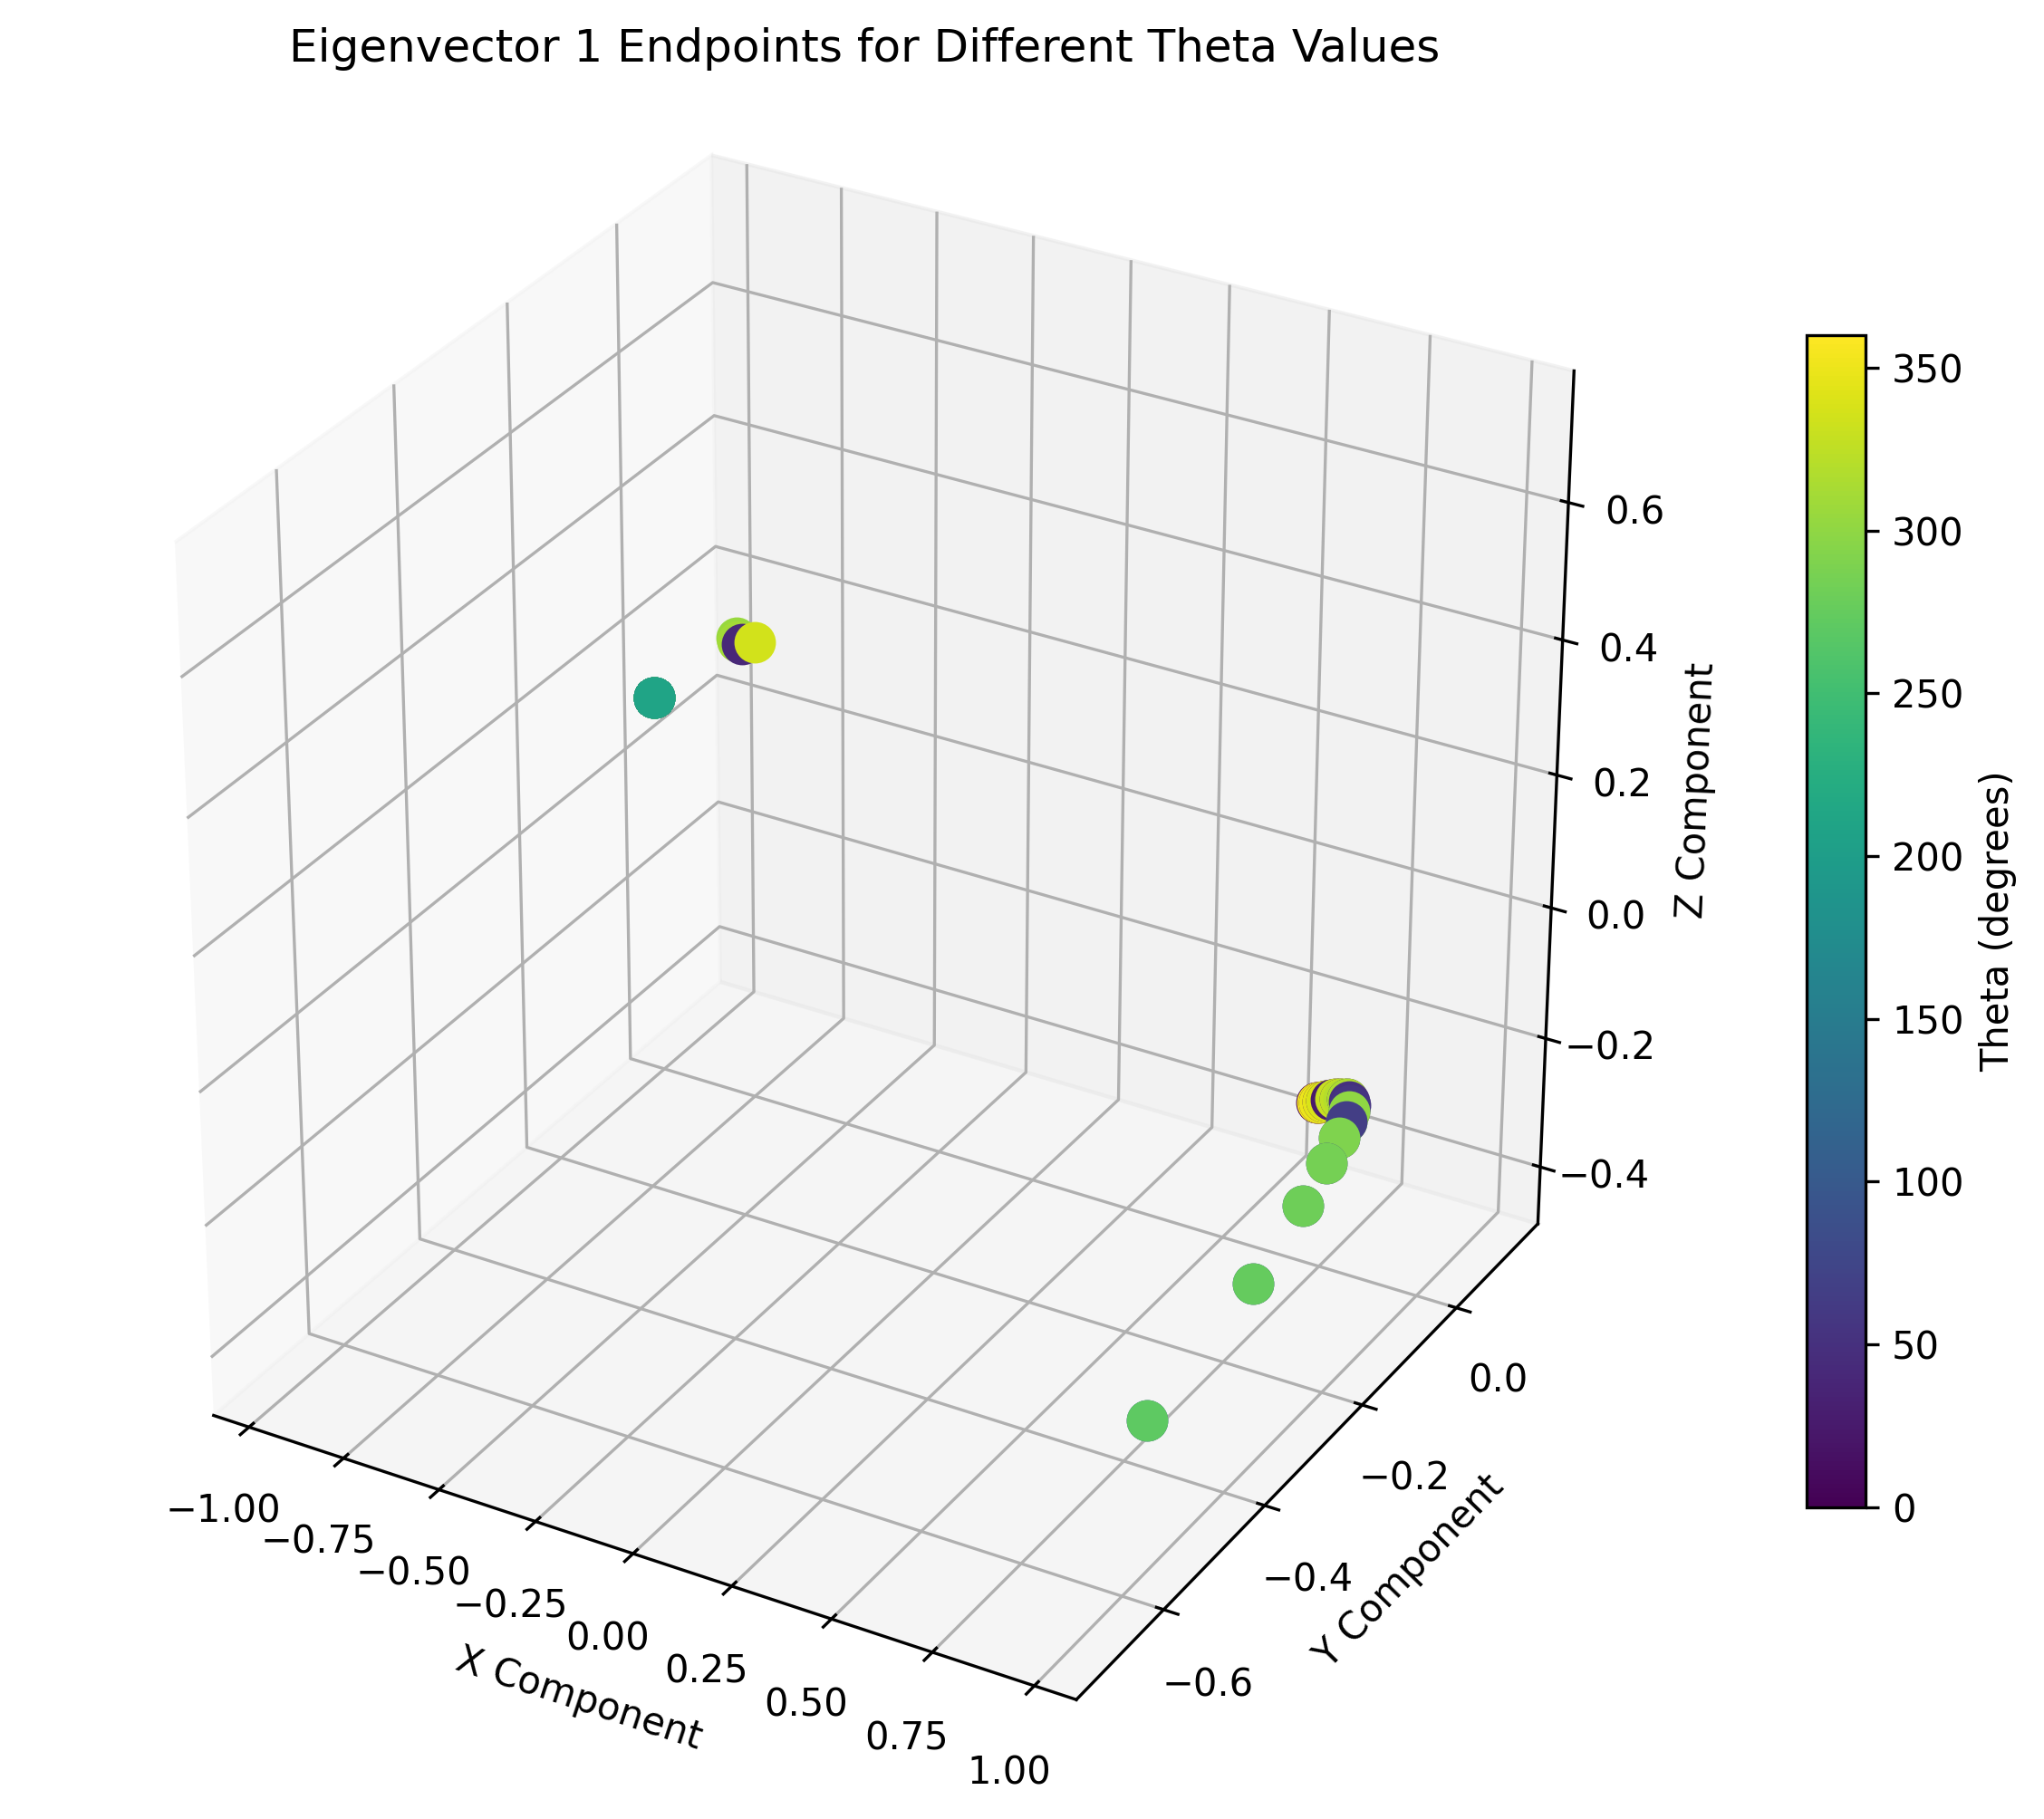
\includegraphics[width=0.8\textwidth]{../example_use/arrowhead_matrix/results/plots/eigenvector_1_no_labels.png}
    \caption{Second eigenvector endpoints for different $\theta$ values}
    \label{fig:eigenvector_1_no_labels_gen}
\end{figure}

\begin{figure}[H]
    \centering
    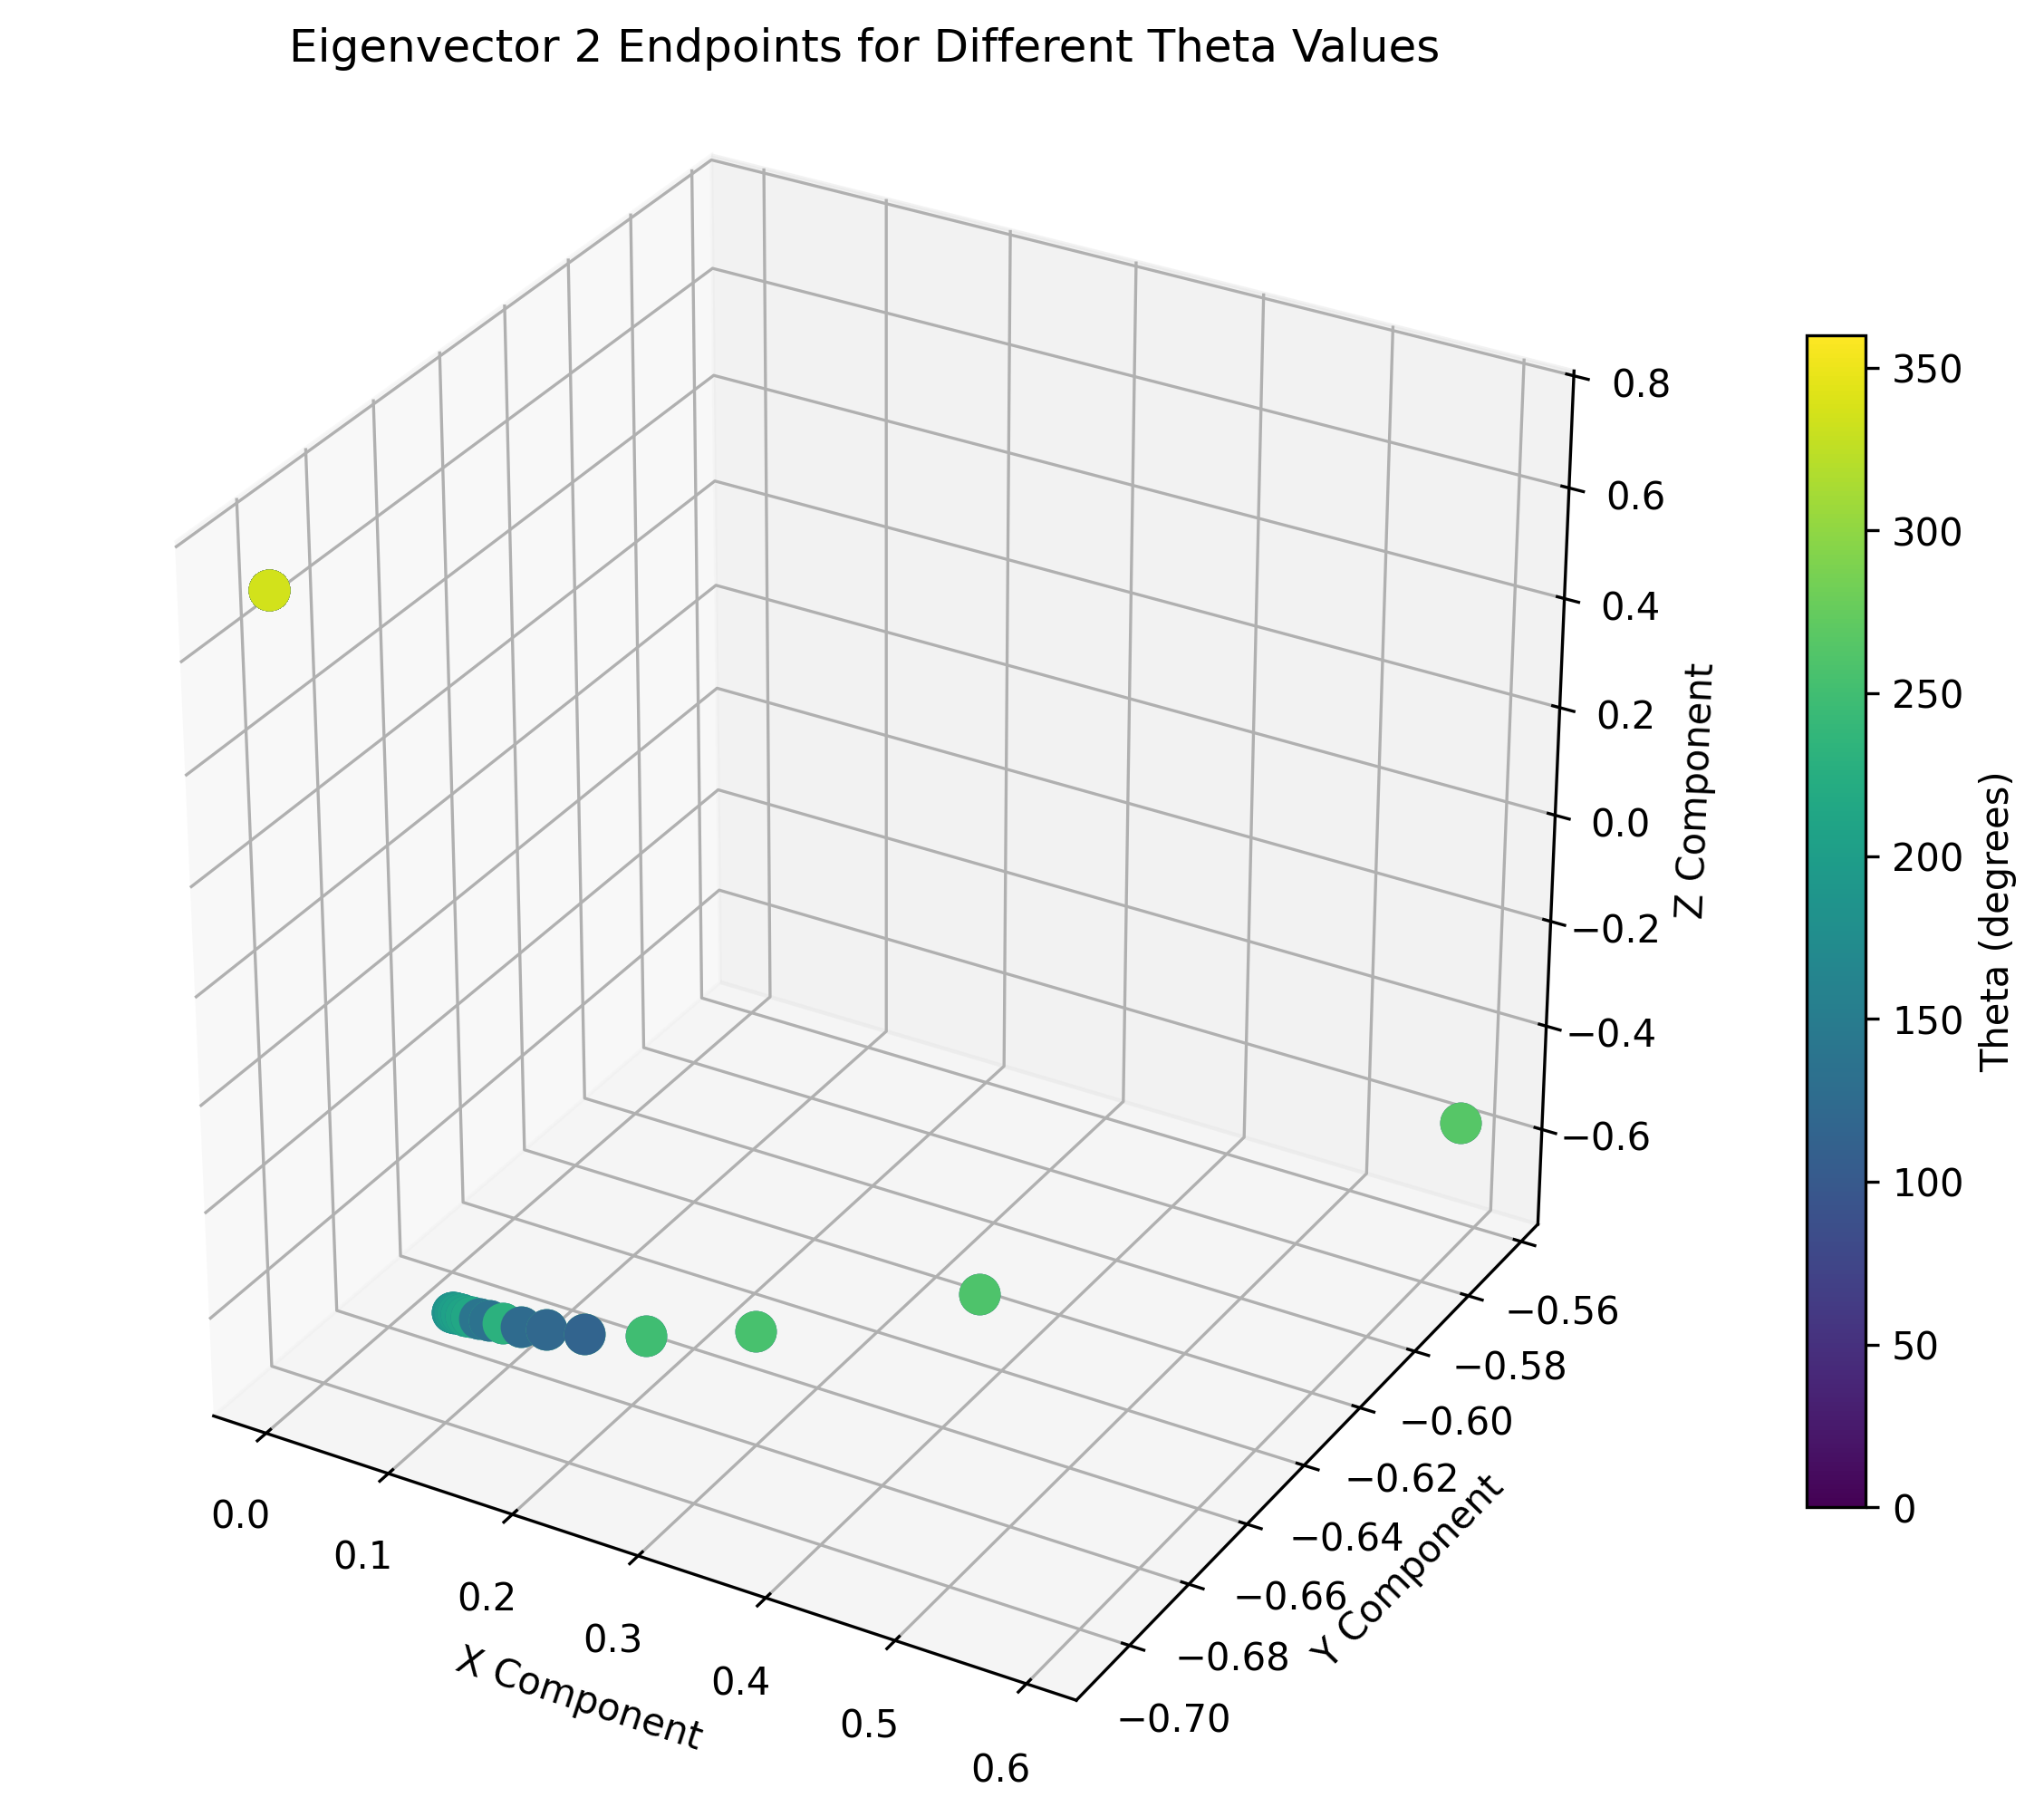
\includegraphics[width=0.8\textwidth]{../example_use/arrowhead_matrix/results/plots/eigenvector_2_no_labels.png}
    \caption{Third eigenvector endpoints for different $\theta$ values}
    \label{fig:eigenvector_2_no_labels_gen}
\end{figure}

\begin{figure}[H]
    \centering
    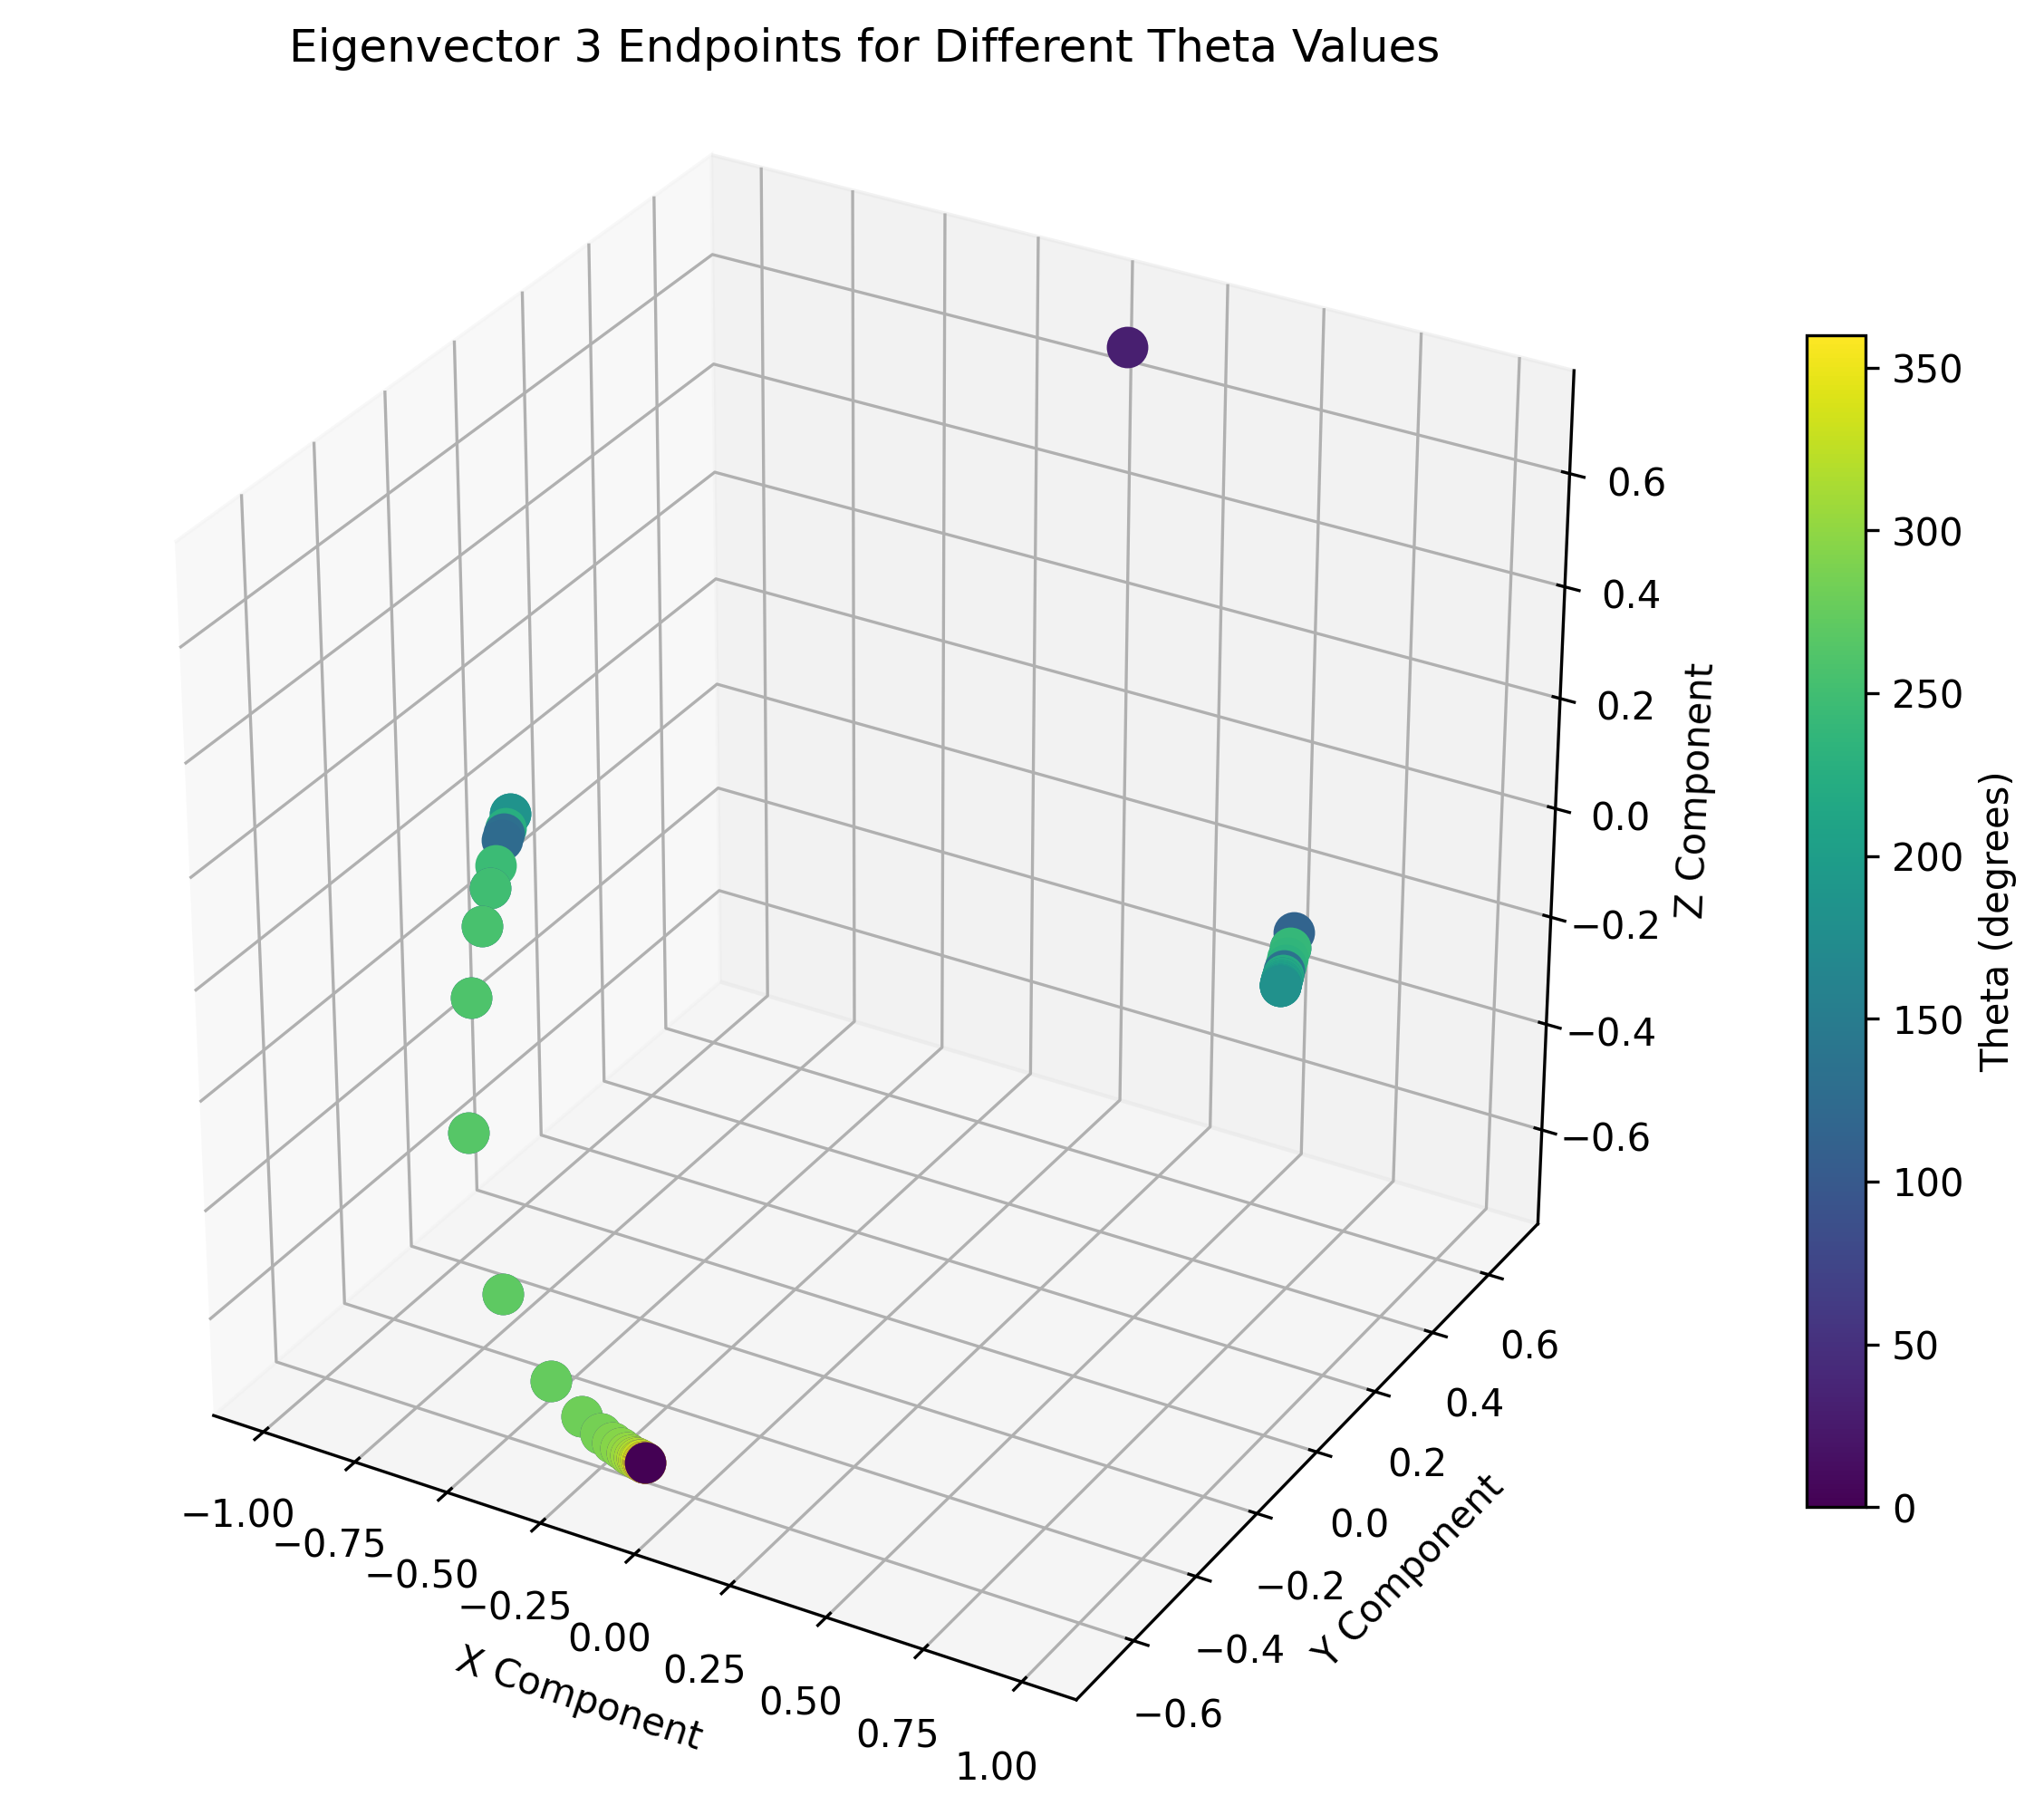
\includegraphics[width=0.8\textwidth]{../example_use/arrowhead_matrix/results/plots/eigenvector_3_no_labels.png}
    \caption{Fourth eigenvector endpoints for different $\theta$ values}
    \label{fig:eigenvector_3_no_labels_gen}
\end{figure}

\subsubsection{R Vectors Visualization}

Figure \ref{fig:r_vectors_3d_gen} shows the R vectors for different values of $\theta$, forming a perfect circle in the plane orthogonal to the x=y=z line.

\begin{figure}[H]
    \centering
    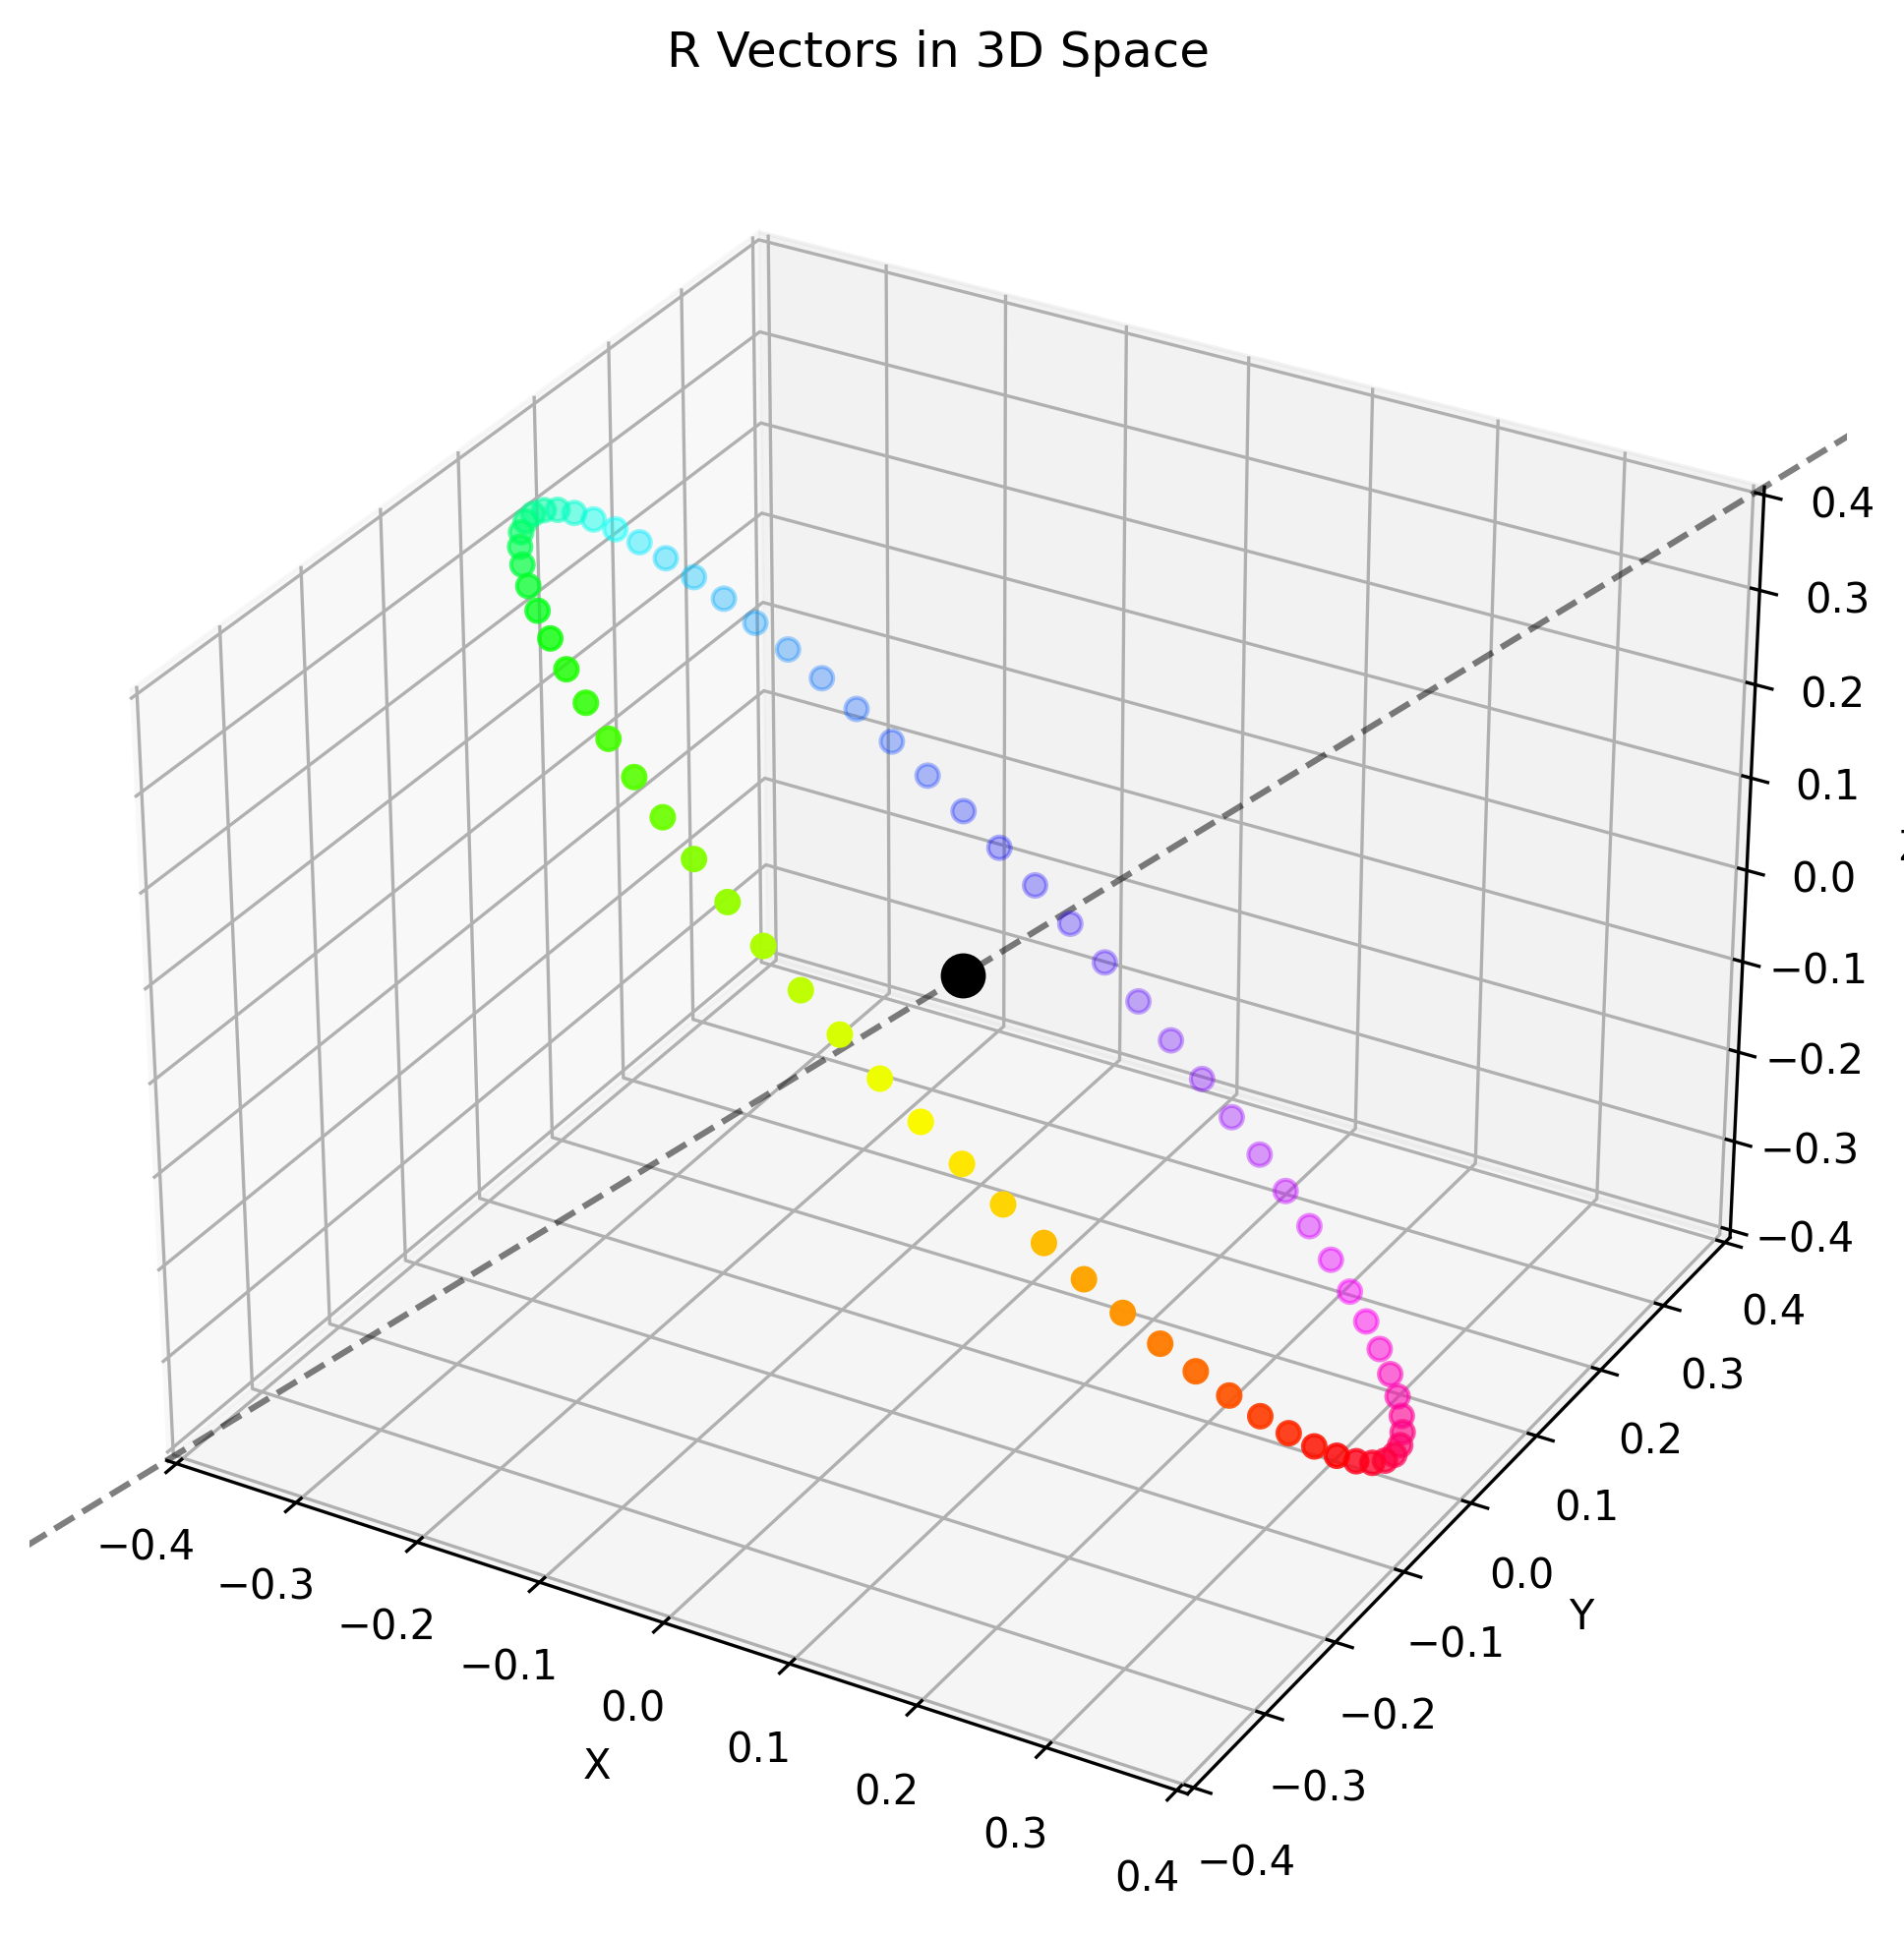
\includegraphics[width=0.8\textwidth]{../example_use/arrowhead_matrix/results/plots/r_vectors_3d.png}
    \caption{R vectors forming a circle in 3D space}
    \label{fig:r_vectors_3d_gen}
\end{figure}

\subsection{Source Code}

The complete source code for the generalized arrowhead matrix implementation is provided in the appendix. The main script, \texttt{arrowhead.py}, is shown below:

\begin{verbatim}
#!/usr/bin/env python3
"""
Arrowhead Matrix Generator and Analyzer

This script provides a unified interface for generating, analyzing, and visualizing
arrowhead matrices. It combines the functionality of the separate scripts into a
single, easy-to-use tool.

Features:
- Generate arrowhead matrices of any size
- Calculate eigenvalues and eigenvectors
- Create 2D and 3D visualizations
- Save results in organized directories
"""

import sys
import os
import numpy as np
import matplotlib.pyplot as plt
from scipy import linalg
import argparse
from mpl_toolkits.mplot3d import Axes3D

# Add the parent directory to the path so we can import the modules
sys.path.append(os.path.abspath(os.path.join(os.path.dirname(__file__), '../..')))
from vector_utils import create_perfect_orthogonal_vectors, generate_R_vector

# Import local modules
from file_utils import organize_results_directory, get_file_path
from generate_arrowhead_matrix import ArrowheadMatrix
from generate_4x4_arrowhead import ArrowheadMatrix4x4
from plot_improved import plot_eigenvalues_2d, plot_eigenvectors_no_labels


class ArrowheadMatrixAnalyzer:
    """
    A unified class for generating, analyzing, and visualizing arrowhead matrices.
    """
    
    def __init__(self, 
                 R_0=(0, 0, 0), 
                 d=0.5, 
                 theta_start=0, 
                 theta_end=2*np.pi, 
                 theta_steps=72,
                 coupling_constant=0.1, 
                 omega=1.0, 
                 matrix_size=4, 
                 perfect=True,
                 output_dir=None):
        """
        Initialize the ArrowheadMatrixAnalyzer.
        """
        # ... (initialization code) ...
        
    def generate_matrices(self):
        """
        Generate arrowhead matrices for all theta values.
        """
        # ... (matrix generation code) ...
        
    def calculate_eigenvalues_eigenvectors(self):
        """
        Calculate eigenvalues and eigenvectors for all matrices.
        """
        # ... (eigenvalue calculation code) ...
        
    def load_results(self):
        """
        Load previously calculated eigenvalues and eigenvectors.
        """
        # ... (result loading code) ...
        
    def create_plots(self):
        """
        Create plots for eigenvalues and eigenvectors.
        """
        # ... (plotting code) ...
    
    def plot_r_vectors(self):
        """
        Create a 3D plot of the R vectors.
        """
        # ... (R vector plotting code) ...
    
    def run_all(self):
        """
        Run the complete analysis pipeline.
        """
        # ... (pipeline code) ...


def main():
    """
    Main function to parse command line arguments and run the analysis.
    """
    # ... (command-line argument parsing and execution code) ...


if __name__ == "__main__":
    main()
\end{verbatim}

The full implementation can be found in the \texttt{arrowhead.py} file in the \texttt{example\_use/arrowhead\_matrix} directory.

\subsection{Conclusion}

The generalized arrowhead matrix implementation provides a powerful and flexible tool for generating, analyzing, and visualizing arrowhead matrices. By combining the functionality of multiple scripts into a single, easy-to-use interface, it simplifies the process of working with these matrices and enables more efficient exploration of their properties.

The implementation is designed to be extensible, allowing for matrices of any size to be generated and analyzed. It also provides comprehensive visualization capabilities, making it easier to understand the behavior of the eigenvalues and eigenvectors as the theta parameter varies.

This generalized implementation represents a significant improvement over the previous approach, providing a more unified and user-friendly experience while maintaining all the functionality of the original scripts.
